\section{深度学习}
本章介绍了深度学习的应用案例研究,深度学习是使用人工神经网络的机器学习的最新分支。 
机器学习已被用于许多应用领域,根据从数据集中收集的经验来训练或调整应用程序逻辑。 
为了有效,人们通常需要使用大量数据进行此类训练。 
虽然机器学习作为计算机科学的一个学科已经存在很长时间了,但由于两个原因,它最近在实际行业中获得了广泛的认可。 
第一个原因是互联网的普遍使用提供了大量数据。 
第二个原因是廉价的大规模并行 GPU 计算系统,可以利用这些海量数据集有效地训练应用程序逻辑。 
我们将从机器学习和深度学习的简要介绍开始,然后更详细地考虑最流行的深度学习算法之一:卷积神经网络(CNN)。 
CNN 具有较高的计算与内存访问比率和高水平的并行性,这使它们成为 GPU 加速的完美候选者。 
我们将首先介绍卷积神经网络的基本实现。 接下来,我们将展示如何使用共享内存改进这个基本实现。 
然后,我们将展示如何将卷积层表示为矩阵乘法,这可以通过在现代 GPU 中使用高度优化的硬件和软件来加速。

\subsection{背景}
机器学习是 IBM 的 Arthur Samuel 于 1959 年创造的术语 (Samuel, 1959),是计算机科学的一个领域,
研究从数据中学习应用程序逻辑的方法,而不是设计显式算法。 
机器学习在设计显式算法不可行的计算任务中最为成功,主要是因为在设计此类显式算法时没有足够的知识。 
也就是说,人们可以给出在各种情况下应该发生什么的例子,但不能给出针对所有可能的输入做出此类决策的一般规则。 
例如,机器学习促进了自动语音识别、计算机视觉、自然语言处理和推荐系统等应用领域的最新改进。 
在这些应用领域中,人们可以提供许多输入示例以及每个输入应该产生什么结果,但没有一种算法可以正确处理所有可能的输入。

使用机器学习创建的应用程序逻辑类型可以根据它们执行的任务类型进行组织。 机器学习任务种类繁多。 
在这里,我们展示了众多中的一些:
\begin{itemize}
   \item 分类:确定输入属于 $k$ 类别中的哪一个。 一个例子是对象识别,例如确定照片中显示的食物类型。

   \item 回归:预测给定一些输入的数值。 一个例子是预测下一个交易日结束时股票的价格。

   \item 转录:将非结构化数据转换为文本形式。 一个例子是光学字符识别。

   \item 翻译:将一种语言的符号序列转换为另一种语言的符号序列。 一个例子是从英语翻译成中文。

   \item 嵌入:将输入转换为向量,同时保留实体之间的关系。 一个例子是将自然语言句子转换为多维向量。

\end{itemize}

读者可以参考大量有关机器学习各种任务的数学背景和实用解决方案的文献。 
本章的目的是介绍分类任务的神经网络方法中涉及的计算内核。 
对这些内核的具体理解将使读者能够理解和开发用于其他机器学习任务的深度学习方法的内核。 
因此,在本节中,我们将详细介绍分类任务,以建立理解神经网络所需的背景知识。 
从数学上讲,分类器是一个函数 $f$,它将输入映射到 $k$ 类别或标签:
$$
f: R^{n} \rightarrow\{1,2, \ldots, k\}
$$

函数$f$由$\theta$参数化,将输入向量$\mathrm{x}$映射到数字代码$y$,即
$$
y=f(x, \theta)
$$

参数 $\theta$ 通常称为模型。 它封装了从数据中学习到的权重。 $\theta$ 的定义最好用一个具体的例子来说明。 
让我们考虑一个称为感知器的线性分类器(Rosenblatt,1957):$y=\operatorname{sign}(W \cdot x+b)$,
其中 $\mathrm{W}$ 是与以下长度相同的权重向量 $x$ 和 $b$ 是偏差常数。 
如果输入为正,则 Sign 函数返回值 1;如果输入为 0,则返回 0;如果输入为负,则返回 -1。 
也就是说,作为分类器的符号函数激活(即最终确定)输入值到三个类别的映射:$\{-1,0,1\}$; 因此它通常被称为激活函数。 
激活函数将非线性引入感知器的线性函数中。 在这种情况下,模型 $\theta$ 是向量 $W$ 和常数 $b$ 的组合。 
模型的结构是一个符号函数,其输入是输入 $x$ 元素的线性表达式,其中系数是 $W$ 的元素,常数是 $b$。

\begin{figure}[H]
	\centering
	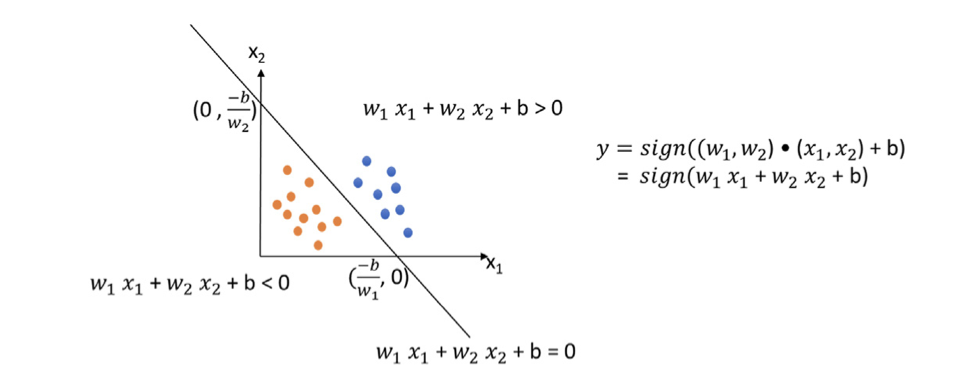
\includegraphics[width=0.9\textwidth]{figs/F16.1.png}
	\caption{\textit{感知器线性分类器示例,其中输入是二维向量。}}
\end{figure}

图 16.1 显示了一个感知器示例,其中每个输入都是二维 (2D) 向量 $\left(x_{1}, x_{2}\right)$。 
线性感知器的模型$\theta$由权重向量$\left(w_{1}, w_{2}\right)$和偏差常数$b$组成。 
如图 16.1 所示,线性表达式 $w_{1} x_{1}+w_{2} \cdot x_{2}+b$ 
定义了 $x_{1}-x_{2}$ 空间中的一条线 它将空间分成两部分:所有点都使表达式大于零的部分和所有点都使表达式小于零的部分。 
线上的所有点都使表达式等于 0 。

视觉上,给定 $\left(w_{1}, w_{2}\right)$ 和 $b$ 值的组合,
我们可以在 $\left(x_{1}, x_{2}\right)$空间,如图16.1所示。 
例如,对于模型为 $\left(w_{1}, w_{2}\right)=(2,3)$ 和 $b=-6$ 的感知器,
我们可以通过连接两者轻松画一条线 与 $x_{1}$ 轴 $\left(\left(\frac{-b}{w_{1}}, 0\right)=(3,0)\right)$ 
和 $x_{2}$轴的交点$\left(\left(0, \frac{-b}{w_{2}}\right)=(0,2)\right)$. 
由此绘制的线对应于方程 $2 x_{1}+3 x_{2}-6$ $=0$ 通过此图,我们可以轻松可视化输入点的结果: 
线上方的任何点(显示为蓝点 图 16.1 中的点)被分类为 1 类,线上的任意点被分类为 0 类,
线下方的任意点(如图 16.1 中的橙色点所示)被分类为 -1 类。

计算输入的类别的过程通常称为分类器的推理。 
对于感知器,我们只需将输入坐标值插入 $y=\operatorname{sign}(W \cdot x+b)$ 中。 
在我们的例子中,如果输入点是$(5,-1)$,我们可以通过将其坐标插入感知器函数来进行推理:
$$
y=\operatorname{sign}(2 * 5+3 *(-1)+6)=\operatorname{sign}(13)=1
$$

因此 $(5,-1)$ 被分类为 1 类,即位于蓝点之中。

\subsubsection{多层分类器}
当有一种方法可以绘制超平面(即 $2 \mathrm{D}$ 空间中的线和三维 [3D] 空间中的平面)
并将空间划分为区域并从而定义每个类别时,线性分类器非常有用。 数据点。 
理想情况下,每一类数据点应该恰好占据一个这样的区域。 
例如,在 2D、2 类分类器中,我们需要能够绘制一条线,将一类的点与另一类的点分开。 不幸的是,这并不总是可行。

\begin{figure}[H]
	\centering
	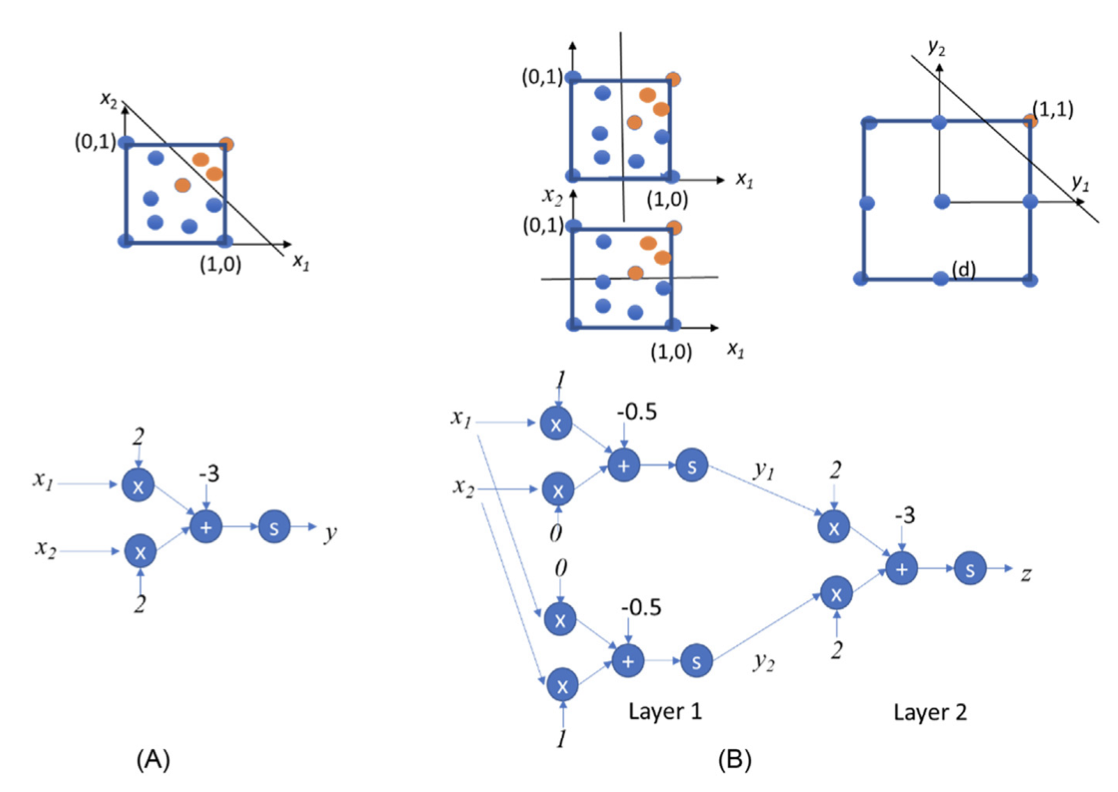
\includegraphics[width=0.9\textwidth]{figs/F16.2.png}
	\caption{\textit{多层感知器示例。}}
\end{figure}

考虑图 16.2 中的分类器。 假设所有输入的坐标都在$[0,1]$范围内。 
分类器应将 $x_{1}$ 和 $x_{2}$ 值均大于 0.5 的所有点(落在域右上象限的点)分类为 1 类,其余分类为 -1 类。 
该分类器可以近似地用如图 16.2(A) 所示的线来实现。 例如,行 $2 x_{1}+2 x_{2}-3=0$ 可以正确分类大多数点。 
然而,一些$x_{1}$和$x_{2}$都大于0.5但总和小于1.5的橙色点,例如$(0.55,0.65)$,会被错误分类到类中 -1(蓝色)。 
这是因为任何线都必然要么切除右上象限的一部分,要么包含域的其余部分的一部分。 没有一条线可以正确分类所有可能的输入。

多层感知器 (MLP) 允许使用多条线来实现更复杂的分类模式。 在多层感知器中,每一层都由一个或多个感知器组成。 
一层感知器的输出是下一层感知器的输入。 
一个有趣且有用的属性是,虽然第一层的输入具有无限数量的可能值,但第一层的输出以及第二层的输入只能具有适度数量的可能值。 
例如,如果图 16.1 中的感知器用作第一层,则其输出将被限制为 $\{-1,0,1\}$。

图16.2(B)显示了一个两层感知器,可以精确地实现所需的分类模式。 第一层由两个感知器组成。 
第一个 $y_{1}=\operatorname{sign}\left(x_{1}-0.5\right)$ 将所有 $x_{1}$ 坐标大于 0.5 的点分类为 1 类; 
即输出值为 1 。 其余点被分类为 -1 类或 0 类。 
第一层中的第二个分类器 $y_{2}=\operatorname{sign}\left(x_{2}-0.5\right)$ 将所有 $x_{2}$ 坐标大于 0.5 的点分类为类 1. 其余的点被分类为-1 类。

因此第一层的输出$\left(y_{1}, y_{2}\right)$只能是以下九种可能之一:$(-1,-1)$,$(-1,0)$, $(-1,1)$,$(0,-1)$, 
$(0,0)$, $(0,1)$, $(1,-1)$,$(1,0)$,$(1,1)$。 
也就是说,第二层只有九个可能的输入对值。 在这九种可能性中,$(1,1)$ 是特殊的。 
橙色类别中的所有原始输入点都被第一层映射到$(1,1)$。 
因此,我们可以在第二层使用一个简单的感知器在$(1,1)$和$y_{1}-y_{2}$空间中的其他八个可能的点之间画一条线,
如图16.2B所示 。 这可以通过 $2 y_{1}+2 y_{2}-3=0$ 行或许多其他行(它的小变体)来完成。

让我们使用图 16.2A 中单层感知器错误分类的 $(0.55,0.65)$ 输入。 
当经过两层感知器处理时,图16.2B中第一层的上感知器生成$y_{1}=1$,下感知器生成$y_{2}=1$。 
根据这些输入值,第二层中的感知器生成 $z=1$,即 $(0.55,0.65)$ 的正确分类。

\begin{figure}[H]
	\centering
	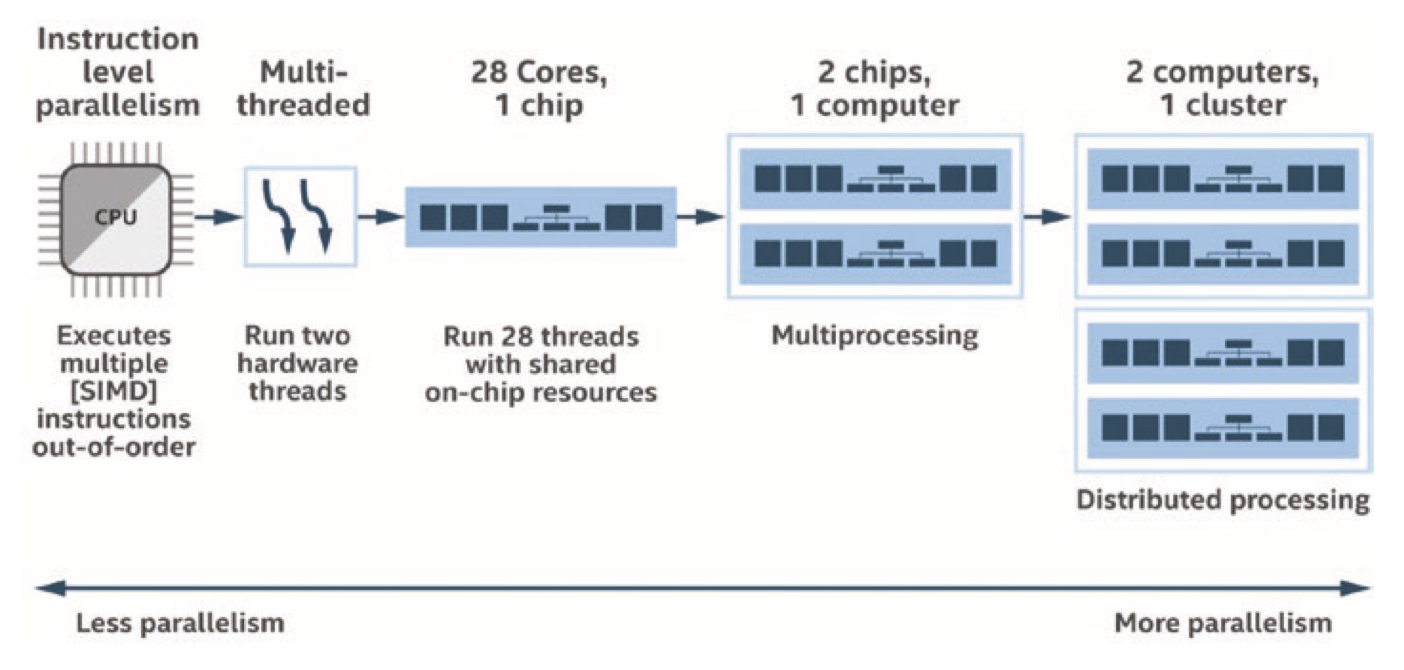
\includegraphics[width=0.9\textwidth]{figs/F16.3.png}
	\caption{\textit{需要两层以上的感知器。}}
\end{figure}

请注意,两层感知器仍然具有很大的局限性。 例如,假设我们需要构建一个感知器来对图 16.3A 所示的输入点进行分类。 
橙色输入点的值可以导致第二层的输入值 $(-1,-1)$ 或 $(1,1)$。 我们看到没有办法画一条线来正确分类第二层中的点。 
我们在图 16.2B 中表明,我们可以通过在第二层添加另一个感知器来添加另一条线。 
该函数将是 $z_{2}=\operatorname{sign}\left(-2 y_{1}-2 y_{2}-3\right)$ 或其较小的变体。 
读者应该验证图 16.3B 中的所有蓝点都将映射到 $z_{1}-z_{2}$ 空间中的 $(-1,-1)$。 
而 $y_{1}-y_{2}$ 空间中的 $(1,1)$ 和 $(-1,-1)$ 映射到 $(1,-1)$ 和 $(-1,1 )$ 在 $z_{1}-z_{2}$ 空间中。 
现在我们可以画一条线 $z_{1}+z_{2}+1=0$ 或其微小变化来正确分类点,如图 16.3C 所示。 
显然,如果我们需要将输入域划分为更多区域,我们可能需要更多层来执行正确的分类。

图 16.2B 中的第 1 层是全连接层的一个小示例,其中每个输出(即 $\quad y_{1}, y_{2}$ )都是每个输入(即 $x_{ 1},x_{2}$)。 
一般来说,在全连接层中,每一个 $m$ 输出都是所有 $n$ 输入的函数。 
全连接层的所有权重形成$\mathrm{m} \times \mathrm{n}$权重矩阵$\mathrm{W}$,
其中$\mathrm{m}$的每一行都是权重向量 (大小为 $\mathrm{n}$ 元素)应用于输入向量(大小为 $n$ 元素)
以生成 $m$ 输出之一。 因此,从全连接层的输入评估所有输出的过程是矩阵向量乘法。 
正如我们将看到的,全连接层是许多类型神经网络的核心组件,我们将进一步研究 GPU 实现。

当 $m$ 和 $n$ 变大时,完全连接的层变得极其昂贵。 主要原因是全连接层需要 $m \times n$ 权重矩阵。 
例如,在图像识别应用中,$n$是输入图像中的像素数量,$\mathrm{m}$是需要对输入像素执行分类的数量。 
在这种情况下,对于高分辨率图像,$\mathrm{n}$ 为数百万,而 $\mathrm{m}$ 可以为数百或更多,
具体取决于需要识别的对象的种类。 此外,图像中的对象可以具有不同的尺度和方向; 可能需要使用许多分类器来处理这些变化。 
向所有这些分类器提供所有输入既昂贵又可能造成浪费。 
卷积层通过减少每个分类器采用的输入数量并在分类器之间共享相同的权重来降低全连接层的成本。 
在卷积层中,每个分类器仅获取输入图像的一个块,并根据权重对块中的像素执行卷积。 
输出称为输出特征图,因为输出中的每个像素都是分类器的激活结果。 
跨分类器共享权重允许卷积层拥有大量分类器,即大的 $\mathrm{m}$ 值,而无需过多的权重。 
在计算上,这可以实现为二维卷积。 然而,这种方法有效地将相同的分类器应用于图像的不同部分。 
我们可以将不同的权重集应用于同一输入并生成多个输出特征图,正如我们将在本章后面看到的那样。

\subsubsection{训练模型}
到目前为止,我们假设分类器使用的模型参数以某种方式可用。 
现在我们转向训练,或者使用数据来确定模型参数 $\theta$ 值的过程,包括权重 $\left(w_{1}, w_{2}\right)$ 和偏差 $b $。 
为简单起见,我们将假设监督训练,其中标有所需输出值的输入数据用于确定权重和偏差值。 
其他训练方式,例如半监督学习和强化学习,也被开发出来以减少对标记数据的依赖。 
读者可以参考文献来了解如何在这种情况下完成训练。

\subsubsection{误差函数}
一般来说,训练将模型参数视为未知变量,并在给定标记输入数据的情况下解决逆问题。 
在图 16.1 的感知器示例中,用于训练的每个数据点都将标有其所需的分类结果: $-1,0$ 或 1 。 
训练过程通常从 $\left(w_{1}, w_{2}\right)$ 和 $b$ 值的初始猜测开始,并对输入数据进行推理并生成分类结果。 
将这些分类结果与标签进行比较。 误差函数(有时称为成本函数)被定义为量化每个数据点的分类结果与相应标签之间的差异。 
例如,假设 $y$ 是分类输出类,$t$ 是标签。 以下是误差函数示例:

$$
E=\frac{(y-t)^{2}}{2}
$$

该误差函数有一个很好的特性,即只要 $y$ 和 $t$ 的值之间存在任何差异(正数或负数),误差值就始终为正。 
如果我们需要对许多输入数据点的误差求和,则正差和负差都会对总和产生影响,而不是相互抵消。 
在许多其他选项中,人们还可以将误差定义为差异的绝对值。 
正如我们将看到的,系数 $\frac{1}{2}$ 简化了求解模型参数所涉及的计算。

\subsubsection{随机梯度下降}
训练过程将尝试找到使所有训练数据点的误差函数值之和最小化的模型参数值。 
这可以通过随机梯度下降方法来完成,该方法通过分类器重复运行输入数据集的不同排列,演化参数值,
并检查参数值是否已经收敛,因为它们的值已经稳定并且变化小于阈值 最后一次迭代。 一旦参数值收敛,训练过程就结束。

\subsubsection{Epoch}
在训练过程的每次迭代(称为纪元)期间,训练输入数据集在输入到分类器之前首先会被随机打乱(即排列)。 
输入数据排序的这种随机化有助于避免次优解决方案。 
对于每个输入数据元素,将其分类器输出 $y$ 值与标签数据进行比较以生成误差函数值。 
在我们的感知器示例中,如果数据标签为 (class) 1 并且分类器输出为 (class) -1 ,
则使用 $E=\frac{(y-t)^{2}}{2}$ 的误差函数值为 2. 
如果误差函数值大于阈值,则激活反向传播操作来改变参数,从而可以减少推理误差。

\subsubsection{反向传播}
反向传播的思想是从误差函数开始,回顾分类器并确定每个参数对误差函数值的贡献方式(LeCun 等人,1990)。 
如果当数据元素的参数值增加时误差函数值增加,我们应该减小参数值,以便该数据点的误差函数值可以减小。 
否则,我们应该增加参数值以减少数据点的误差函数值。 
从数学上讲,函数值随着其输入变量之一变化而变化的速率和方向是函数对该变量的偏导数。 
对于感知器,为了计算误差函数的偏导数,模型参数和输入数据点被视为输入变量。 
因此,反向传播操作需要针对触发反向传播操作的每个输入数据元素导出模型参数上的误差函数的偏导数值。

让我们使用感知器 $y=\operatorname{sign}\left(w_{1} x_{1}+w_{2} x_{2}+\mathrm{b}\right)$ 来说明反向传播操作。 
假设误差函数 $E=\frac{(y-t)^{2}}{2}$ 并且反向传播由训练输入数据元素 $(5,2)$ 触发。 
目标是修改 $w_{1}、w_{2}$ 和 $\mathrm{b}$ 值,以便感知器更有可能正确分类 $(5,2)$。 
也就是说,我们需要导出偏导数 $\frac{\partial E}{\partial w_{1}}、\frac{\partial E}{\partial w_{2}}$ 
和 $\frac {\partial E}{\partial b}$ 以便更改 $w_{1}、w_{2}$ 和 $\mathrm{b}$ 值。

\subsubsection{链式法则}
我们看到$E$是$y$的函数,$y$是$w_{1}、w_{2}$和$\mathrm{b}$的函数。 因此我们可以使用链式法则来推导这些偏导数。 
对于 $w_{1}$,
$$
\frac{\partial E}{\partial w_{1}}=\frac{\partial E}{\partial y} \frac{\partial y}{\partial w_{1}}
$$

$\frac{\partial E}{\partial y}$ 很简单:
$$
\frac{\partial E}{\partial y}=\frac{\partial \frac{(y-t)^{2}}{2}}{\partial y}=y-t
$$

然而,我们面临 $\frac{\partial y}{\partial w_{1}}$ 的挑战。 请注意,符号函数不是可微函数,因为它在 0 处不连续。 
为了解决这个问题,机器学习社区通常使用符号函数的更平滑版本,
该版本在零附近可微,并且接近远离 0 的 $\mathrm{x}$ 值的符号函数值。 
这种更平滑版本的一个简单示例是 sigmoid 函数 $s=\frac{1-e^{-x}}{1+e^{-x}}$。 
对于绝对值较大的负数 $x$ 值,sigmoid 表达式以 $e^{-x}$ 项为主,并且 sigmoid 函数值将约为 -1 。 
对于绝对值较大且为正的 $x$ 值,$e^{-x}$ 项会减少,并且函数值将约为 1 。 
对于接近 0 的 $x$ 值,函数值从接近 -1 快速增加到接近 1 。 
因此,sigmoid 函数非常接近符号函数的行为,但对于所有 $x$ 值都是连续可导的。 
从符号变为 sigmoid 后,感知器为 $y=\operatorname{sigmoid}\left(w_{1} x_{1}+w_{2} x_{2}+\mathrm{b}\right)$。 
我们可以将 $\frac{\partial y}{\partial w_{1}}$ 
表示为 $\frac{\partial \operatorname{sigmoid}(k)}{\partial k} \frac{\partial k}{\partial w_{1}}$ 
使用带有中间变量 $k=w_{1} x_{1}+w_{2} x_{2}+\mathrm{b}$ 的链式法则。 
基于微积分操作,$\frac{\partial k}{\partial w_{1}}$ 就是 $x_{1}$ 并且
$$
\begin{aligned}
\frac{\partial \operatorname{sigmoid}(k)}{\partial k} & =\left(\frac{1-e^{-k}}{1+e^{-k}}\right)^ {\prime}=\left(1-e^{-k}\right)^{\prime}\left(\frac{1}{1+e^{-k}}\right)+\left(1 -e^{-k}\right)\left(\frac{1}{1+e^{-k}}\right)^{\prime} \\
& =e^{-k}\left(\frac{1}{1+e^{-k}}\right)+\left(1-e^{-k}\right)\left(-1 \ 次\left(\frac{1}{1+e^{-k}}\right)^{2}\left(-e^{-k}\right)\right)=\frac{2 e^{ -k}}{\left(1+e^{-k}\right)^{2}}
\end{aligned}
$$

把它们放在一起,我们有
$$
\frac{\partial E}{\partial w_{1}}=(y-t) \frac{2 e^{-k}}{\left(1+e^{-k}\right)^{2}} x_{1}
$$

相似地,
$$
\begin{aligned}
\frac{\partial E}{\partial w_{2}} & =(y-t) \frac{2 e^{-k}}{\left(1+e^{-k}\right)^{2} } x_{2} \\
\frac{\partial E}{\partial b} & =(y-t) \frac{2 e^{-k}}{\left(1+e^{-k}\right)^{2}}
\end{aligned}
$$

其中
$$
k=w_{1} x_{1}+w_{2} x_{2}+b
$$

应该清楚的是,所有三个偏导数值都可以通过输入数据 $\left(x_{1}, x_{2}\right.$ 
和 $\left.t\right)$ 的组合来完全确定 模型参数 $\left(w_{1}, w_{2}\right.$ 和 $\left.b\right)$ 的当前值。 
反向传播的最后一步是修改参数值。 回想一下,函数对变量的偏导数给出了当变量改变其值时函数值的变化方向和速率。 
如果给定输入数据和当前参数值的组合,误差函数对参数的偏导数具有正值,我们希望减小参数的值,以便误差函数值减小。 
另一方面,如果变量的误差函数的偏导数具有负值,我们希望增加参数的值,使得误差函数值减小。

\subsubsection{学习率}
数值上,我们希望对误差函数对变化比较敏感的参数进行较大的改变,即当误差函数对该参数的偏导数的绝对值很大时。 
这些考虑因素导致我们从每个参数中减去一个与误差函数对该参数的偏导数成比例的值。 
这是通过将偏导数与常数 $\varepsilon$ 相乘来完成的,该常数在机器学习中称为学习率常数,然后从参数值中减去它。 
$\varepsilon$ 越大,参数值的演化速度越快,因此可以通过更少的迭代来达到解决方案。 
然而,较大的 $\varepsilon$ 也会增加不稳定的可能性并阻止参数值收敛到解决方案。 在我们的感知器示例中,参数的修改如下:
$$
\begin{aligned}
w_{1} & \leftarrow w_{1}-\varepsilon \frac{\partial E}{\partial w_{1}} \\
w_{2} & \leftarrow w_{2}-\varepsilon \frac{\partial E}{\partial w_{2}} \\
b & \leftarrow b-\varepsilon \frac{\partial E}{\partial b}
\end{aligned}
$$

在本章的其余部分中,我们将使用通用符号 $\theta$ 来表示公式和表达式中的模型参数。 
也就是说,我们将用一个通用表达式来表示上面的三个表达式:
$$
\theta \leftarrow \theta-\varepsilon \frac{\partial E}{\partial}
$$

读者应该理解,对于这些通用表达式中的每一个,都可以将 $\theta$ 替换为任何参数,以将表达式应用于参数。

\subsubsection{小批量}
在实践中,由于回溯过程相当昂贵,因此它不是由推理结果与其标签不同的单个数据点触发的。 
相反,在一个时期内对输入进行随机洗牌后,它们被分为称为小批量的片段。 
训练过程通过推理运行整个小批量并累积它们的误差函数值。 如果小批量中的总误差太大,则会触发小批量的反向传播。 
在反向传播过程中,会检查小批量中每个数据点的推理结果,
如果不正确,则使用该数据导出偏导数值,该偏导数值用于修改模型参数值,如上所述。

\subsubsection{训练多层分类器}
对于多层分类器,反向传播从最后一层开始,并修改该层中的参数值,如上所述。 问题是我们应该如何修改前面层的参数。 
请记住,我们可以基于 $\frac{\partial E}{\partial y}$ 推导 $\frac{\partial E}{\partial \theta}$,
正如我们在最后一层所演示的那样。 
一旦我们有了上一层的$\frac{\partial E}{\partial y}$,我们就拥有了计算该层参数修改所需的一切。

一个简单但重要的观察是前一层的输出也是最后一层的输入。 
因此前一层的$\frac{\partial E}{\partial y}$实际上是最后一层的$\frac{\partial E}{\partial x}$。 
因此,关键是在我们修改最后一层的参数值后,导出最后一层的$\frac{\partial E}{\partial x}$。 
如下所示,$\frac{\partial E}{\partial x}$ 与 $\frac{\partial E}{\partial \theta}$ 没有太大区别,
即 $\frac{\partial E}{\partial x}=\frac{\partial E}{\partial y}\frac{\partial y}{\partial x}$。

$\frac{\partial E}{\partial y}$ 可以简单地从参数的推导中重用。 
$\frac{\partial y}{\partial x}$ 也非常简单,因为就 $\mathrm{y}$ 而言,输入与参数起着相同的作用。 
我们只需要对中间函数 $k$ 对输入进行偏导数即可。 对于我们的感知器示例,我们有
$$
\begin{aligned}
& \frac{\partial E}{\partial x_{1}}=(y-t) \frac{2 e^{-k}}{\left(1+e^{-k}\right)^{2} } w_{1} \\
& \frac{\partial E}{\partial x_{2}}=(y-t) \frac{2 e^{-k}}{\left(1+e^{-k}\right)^{2} } w_{2}
\end{aligned}
$$

其中 $k=w_{1} x_{1}+w_{2} x_{2}+$ b. 在图 16.2B 的感知器示例中,最后一层(第 2 层)的 $x_{1}$ 为 $y_{1}$,
第 1 层和 $x_{2}$ 的顶部感知器的输出为 $y_ {2}$,第 1 层底部感知器的输出。 
现在我们准备继续计算上一层两个感知器的$\frac{\partial E}{\partial \theta}$。 显然,如果层数更多,则可以重复此过程。

\subsubsection{前馈网络}
通过连接各层分类器并将每层的输出馈送到下一层,我们形成了一个前馈网络。 图 16.2B 显示了双层前馈网络的示例。 
我们所有关于多层感知器(MLP)的推理和训练的讨论都假设这个属性。 在前馈网络中,前一层的所有输出都进入一个或多个后面的层。 
从后面的层输出到前面的层输入没有连接。 因此,反向传播可以简单地从最后阶段向后迭代,而不会出现反馈循环引起的复杂情况。

\subsection{卷积神经网络}
深度学习过程(LeCun et al., 2015)使用层次结构的特征提取器来学习复杂的特征,
如果有足够的训练数据允许系统正确训练所有层的参数,则可以实现更准确的模式识别结果 特征提取器自动发现足够数量的相关模式。 
有一种深度学习程序比其他程序更容易训练并且可以更好地推广。 
这些深度学习过程基于一种称为卷积神经网络 (CNN) 的特定类型的前馈网络。

CNN 发明于 20 世纪 80 年代末(LeCun 等人,1998)。 
到 20 世纪 90 年代初,CNN 已应用于自动语音识别、光学字符识别 (OCR)、手写识别和人脸识别(LeCun 等,1990)。 
然而,直到 20 世纪 90 年代末,计算机视觉和自动语音识别的主流仍然基于精心设计的功能。 
标记数据量不足以让深度学习系统与人类专家设计的识别或分类功能竞争。 
人们普遍认为,自动构建具有足够层数以比人类定义的特定于应用程序的特征提取器表现更好的分层特征提取器在计算上是不可行的。

2006 年左右,一群研究人员重新燃起了对深度前馈网络的兴趣,
他们引入了无监督学习方法,可以创建多层、分层特征检测器,而不需要标记数据(Hinton 等人,2006 年;Raina 等人,2009 年)。 
这种方法的第一个主要应用是语音识别。 GPU 使这一突破成为可能,它使研究人员训练网络的速度比传统 CPU 快十倍。 
这一进步,加上在线提供的大量媒体数据,极大地提升了深度学习方法的地位。 
尽管在演讲方面取得了成功,但直到 2012 年,CNN 在计算机视觉领域基本上都被忽视了。

2012 年,多伦多大学的一组研究人员训练了一个大型深度卷积神经网络,
用于在 ILSVRC 竞赛中对 1000 个不同类别进行分类(Krizhevsky 等,2012)。 
按照当时的标准,该网络非常庞大:它拥有大约 6000 万个参数和 650,000 个神经元。 
它使用 ImageNet 数据库中的 120 万张高分辨率图像进行训练。 
使用 Alex Krizhevsky(Krizhevsky)编写的基于 CUDA 的卷积神经网络库,该网络仅用一周时间在两个 GPU 上进行了训练。 
该网络取得了突破性的成果,获胜测试错误率为 15.3 \%。 
相比之下,使用传统计算机视觉算法的第二名团队的错误率为 26.2 \%。 
这一成功引发了计算机视觉的革命,CNN成为计算机视觉、自然语言处理、强化学习等许多传统机器学习领域的主流工具。

本节介绍 CNN 推理和训练的顺序实现。 
我们将使用 LeNet-5,该网络是 20 世纪 80 年代末设计的用于数字识别的网络(LeCun 等人,1990)。 
如图16.4所示,LeNet-5由三种类型的层组成:卷积层、子采样层和全连接层。 这三种类型的层仍然是当今神经网络的关键组成部分。 
我们将考虑每种类型层的逻辑设计和顺序实现。 网络的输入显示为灰色图像,其中手写数字表示为 2D $32 \times 32$ 像素阵列。 
最后一层计算输出,即原始图像属于网络设置要识别的十个类别(数字)中每个类别的概率。

\subsubsection{卷积神经网络推理}
\begin{figure}[H]
	\centering
	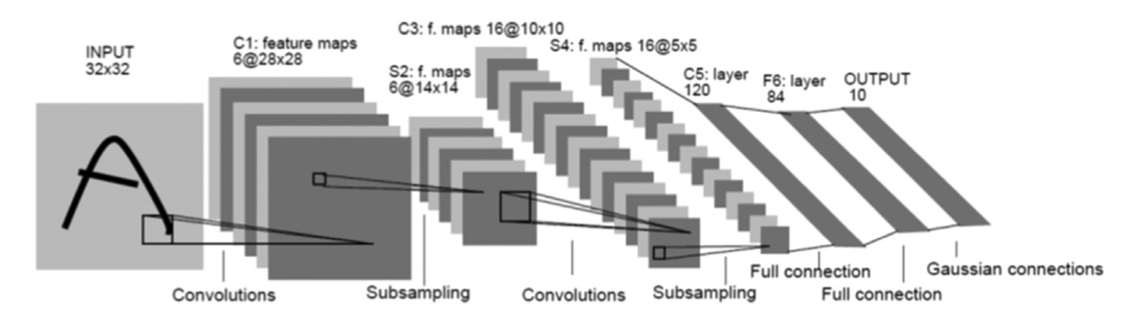
\includegraphics[width=0.9\textwidth]{figs/F16.4.png}
	\caption{\textit{LeNet-5,一种用于手写数字识别的卷积神经网络。 
	输入中的字母 A 不应被分类为十个类别(数字)中的任何一个。}}
\end{figure}

卷积网络中的计算被组织为一系列层。 我们将层的输入和输出称为特征图或简单的特征。 
例如,在图16.4中,网络输入端$\mathrm{C} 1$卷积层的计算被组织为从INPUT像素阵列生成六个输出特征图。 
输入特征图生成的输出由像素组成,每个像素都是通过在前一层(在 C1 的情况下为输入)生成的特征图像素的局部小块和一组权重之间执行卷积而生成的 (即第 7 章:卷积中定义的卷积滤波器)称为滤波器组。 
然后将卷积结果输入到诸如 sigmoid 之类的激活函数中,以在输出特征图中产生输出像素。 
人们可以将输出特征图中每个像素的卷积层视为感知器,其输入是输入特征图中的像素块。 
也就是说,每个输出像素的值是所有输入特征图中对应补丁的卷积结果之和。

\begin{figure}[H]
	\centering
	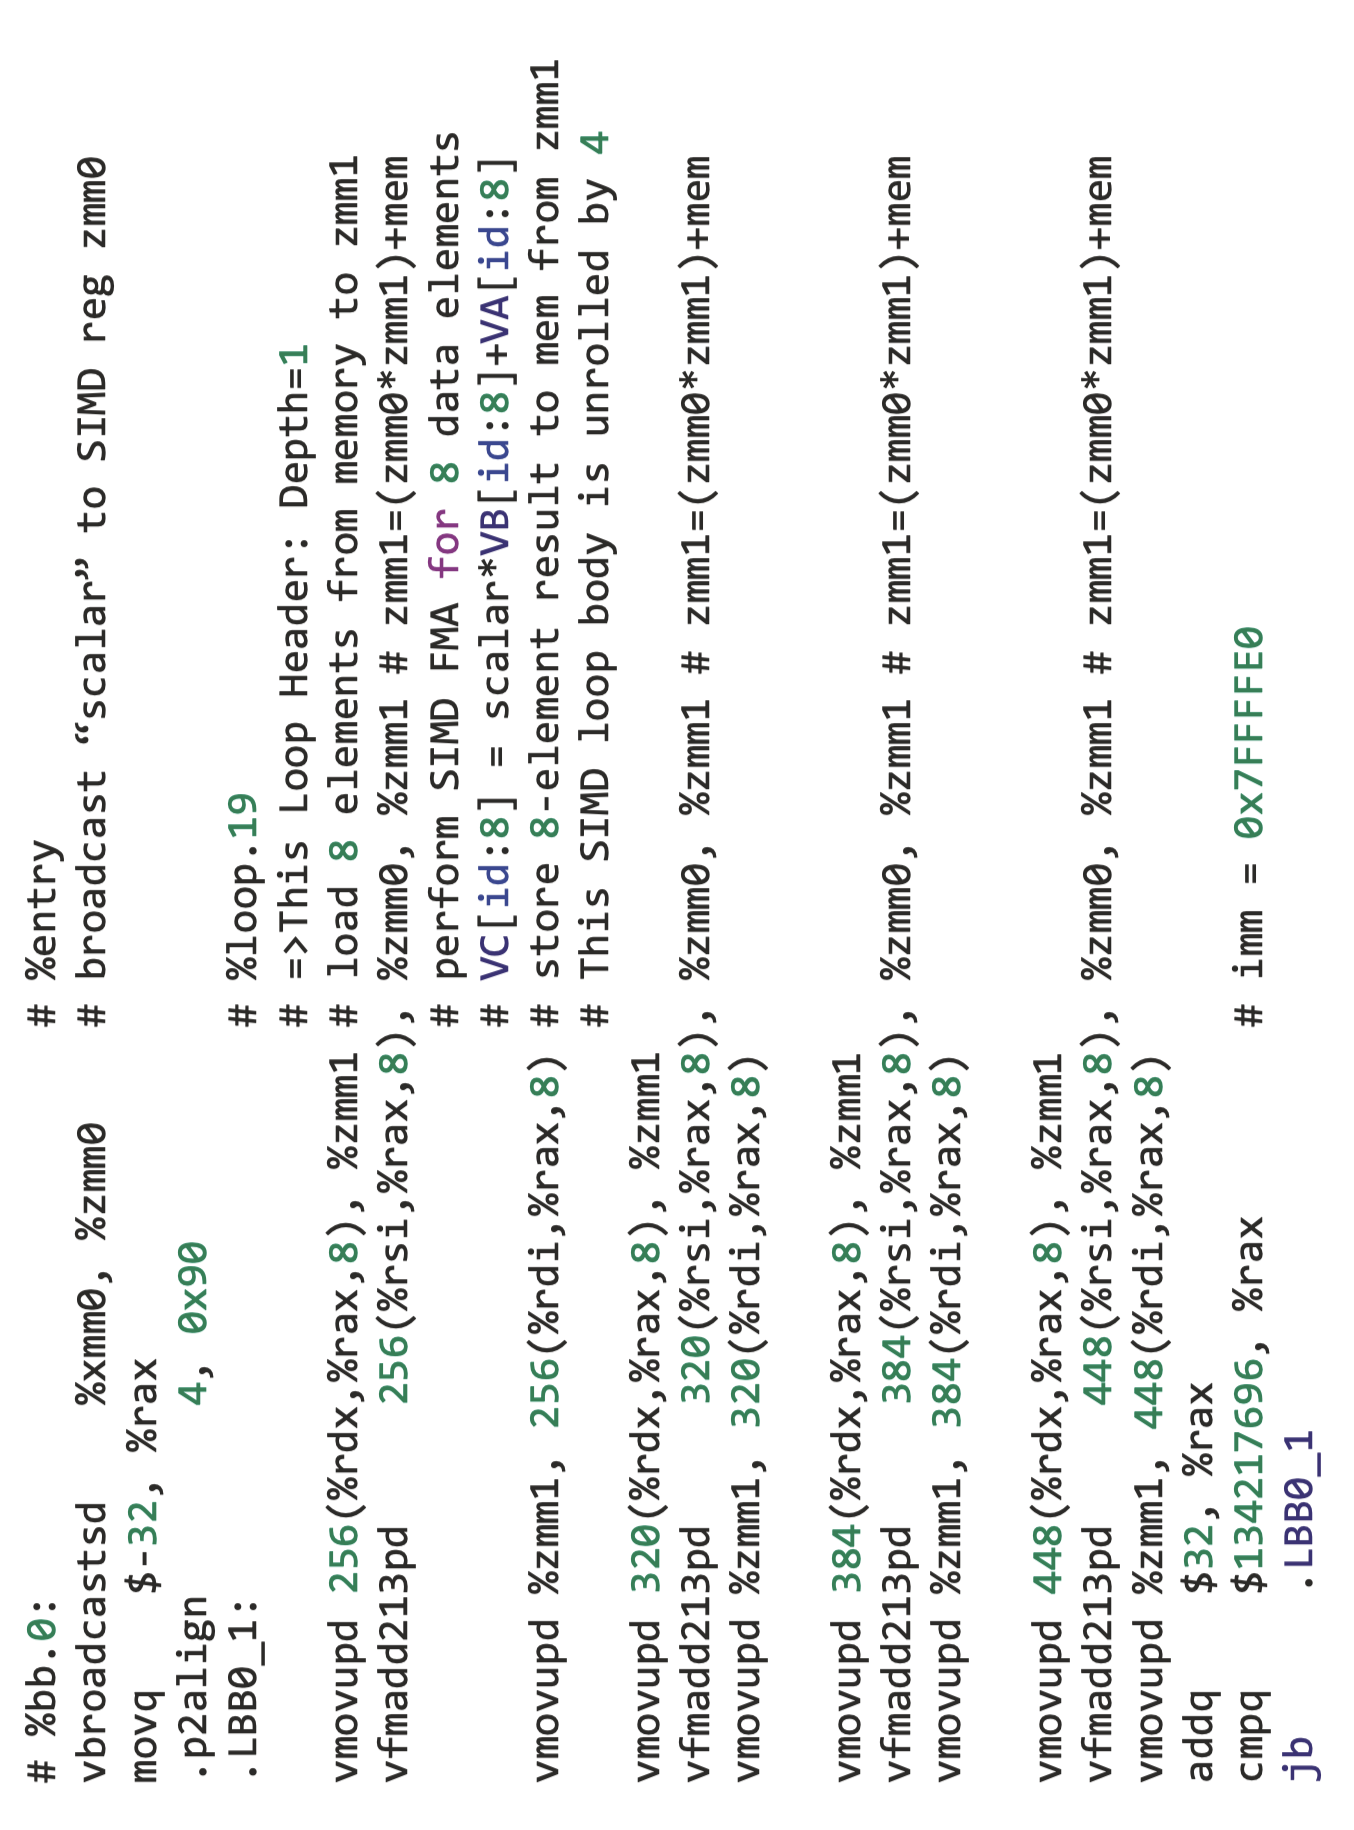
\includegraphics[width=0.9\textwidth]{figs/F16.5.png}
	\caption{\textit{卷积层的前向传播路径。}}
\end{figure}

图 16.5 显示了一个小型卷积层示例。 有三个输入特征图、两个输出特征图和六个滤波器组。 
层中不同对的输入和输出特征图对使用不同的滤波器组。 
由于图 16.5 中有三个输入特征图和两个输出特征图,因此我们需要 $3 \times 2=6$ 滤波器组。 
对于图 16.4 中 LeNet 的 C3 层,有 6 个输入特征图和 16 个输出特征图。 
因此,$\mathrm{C} 3$ 中总共使用了 $6 \times 16=96$ 个滤波器组。

图 16.5B 说明了卷积层完成的计算的更多细节。 为了简单起见,我们省略了输出像素的激活函数。 
我们证明每个输出特征图是所有输入特征图的卷积之和。 
例如,输出特征图 0(值 14)的左上角元素计算为输入特征图的圆圈块与相应滤波器组之间的卷积:
$$
\begin{aligned}
& (1,2,1,1) \cdot(1,1,2,2)+(0,2,0,3) \cdot(1,1,1,1)+(1,2,0, 1) \cdot(0,1,1,0) \\
& =1+2+2+2+0+2+0+3+0+2+0+0 \\
&=14
\end{aligned}
$$

我们还可以将三个输入图视为 3D 输入特征图,将三个滤波器组视为 3D 滤波器组。 
每个输出特征图只是 $3 \mathrm{D}$ 输入特征图和 $3 \mathrm{D}$ 滤波器组的 3D 卷积结果。 
在图16.5B中,左侧的三个2D滤波器组形成3D滤波器组,右侧的三个滤波器组形成第二个3D滤波器组。 
一般来说,如果卷积层有$n$个输入特征图和$m$个输出特征图,则将使用$n^{*} m$个不同的2D滤波器组。 
人们还可以将这些滤波器组视为 $m$ 3D 滤波器组。 
尽管图 16.4 中未显示,但 LeNet-5 中使用的所有 2D 滤波器组都是 $5 \times 5$ 卷积滤波器。 
回想一下第 7 章“卷积”,从输入图像和卷积滤波器生成卷积输出图像需要对“幽灵单元”做出假设。 
LeNet-5 设计没有做出这样的假设,而是简单地使用每个维度边缘的两个元素作为幽灵单元。 
这会将每个维度的大小减少四倍:两个在顶部,两个在底部,两个在左侧,两个在右侧。 
结果,我们看到对于层 $\mathrm{C} 1$,$32 \times 32$ INPUT 图像会产生一个 $28 \times 28$ 图像的输出特征图。 
图 16.4 通过显示 $\mathrm{C} 1$ 层中的像素是从输入像素的方形 $(5 \times 5$,尽管没有明确显示 $)$ 块生成的来说明此计算。

我们假设输入特征图存储在 $3 \mathrm{D}$ 数组 $\mathrm{X}[\mathrm{C}, \mathrm{H}, \mathrm{W}]$ 中,
其中 $\mathrm {C}$是输入特征图的数量,$\mathrm{H}$是每个输入地图图像的高度,$\mathrm{W}$是每个输入地图图像的宽度。 
也就是说,最高维度索引选择特征图之一(通常称为通道),较低二维索引选择输入特征图中的像素之一。 
例如,$\mathrm{C} 1$ 层的输入特征图存储在 $\mathrm{X}$ [1, 32, 32] 中,
因为只有一个输入特征图(图 16.4 中的 INPUT) ),$\mathrm{x}$ 和 $\mathrm{y}$ 维度各包含 32 个像素。 
这也反映了这样一个事实,即我们可以将 2D 输入特征映射到一个层视为形成 3D 输入特征映射。

卷积层的输出特征图也存储在3D数组中 $\mathrm{Y}[\mathrm{M}, \mathrm{H}-\mathrm{K}+1, \mathrm{~W}-\mathrm{K}+1]$,
其中$\mathrm{M}$是输出特征图的数量,$\mathrm{K}$是每个$2\mathrm{D}$过滤器的高度(和宽度)。 
例如,$\mathrm{C} 1$层的输出特征图存储在$\mathrm{Y}[6,28,28]$中,
因为$\mathrm{C} 1$生成六个输出特征图 使用 $5 \times 5$ 过滤器。 
滤波器组存储在四维数组中 $\mathrm{W}[\mathrm{M}, \mathrm{C}, \mathrm{K}, \mathrm{K}]$
\footnote{请注意,W 用于图像的宽度和滤波器组(权重)矩阵的名称。 在每种情况下,其用法都应该从上下文中清楚地看出。} 
有 $\mathrm{M} \times \mathrm{C}$ 个滤波器组。 
滤波器组 $\mathrm{W}\left[\mathrm{m}, \mathrm{c},{ }_{-},\right]$
在使用输入特征图 $\mathrm{X}\left[ 时使用 \mathrm{c},{ }_{-},{ }_{-}\right]$计算输出特征图$\mathrm{Y}[\mathrm{m}$, \textit{,}]。 
回想一下,每个输出特征图是所有输入特征图的卷积之和。 
因此,我们可以将卷积层的前向传播路径视为 $\mathrm{M} 3 \mathrm{D}$ 卷积的集合,
其中每个 3D 卷积由 $3 \mathrm{D}$ 滤波器组指定,
该滤波器组是 $\mathrm{W}$ 的 $\mathrm{C} \times \mathrm{K} \times \mathrm{K}$ 子矩阵。

\begin{figure}[H]
	\centering
	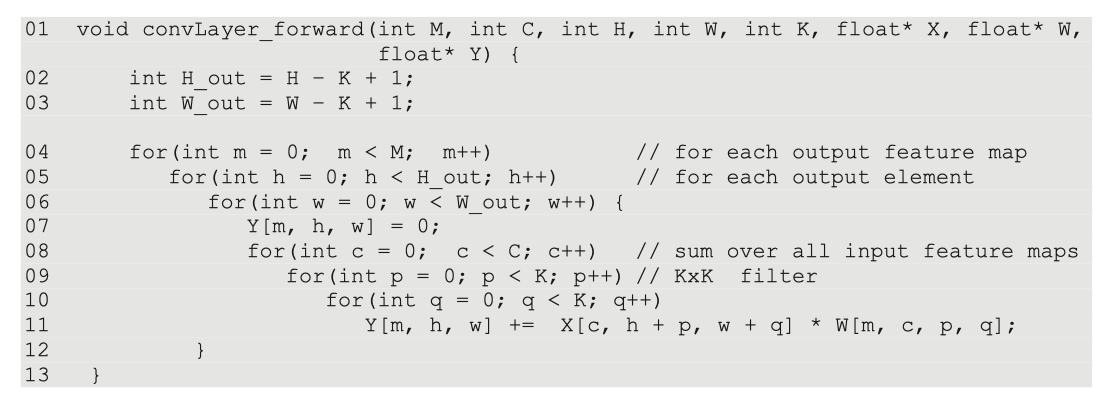
\includegraphics[width=0.9\textwidth]{figs/F16.6.png}
	\caption{\textit{卷积层前向传播路径的 C 实现。}}
\end{figure}

图 16.6 显示了卷积层前向传播路径的顺序 $\mathrm{C}$ 实现。 
最外面的 $(m)$ for 循环(第 04-12 行)的每次迭代都会生成一个输出特征图。 
for 循环(第 05-12 行)的接下来两级( $h$ 和 $w$ )的每次迭代都会生成当前输出特征图的一个像素。 
最里面的三个循环级别(第 08-11 行)在输入特征图和 3D 滤波器组之间执行 3D 卷积。

卷积层的输出特征图通常经过子采样层(也称为池化层)。 子采样层通过组合像素来减小图像图的大小。 
例如,在图16.4中,子采样层S2采用大小为$28×28$的六个输入特征图,并生成大小为$14×14$的六个特征图。 
子采样输出特征图中的每个像素都是从相应输入特征图中的 $2 \times 2$ 邻域生成的。 
这四个像素的值被平均以形成输出特征图中的一个像素。 
下采样层的输出具有与前一层相同数量的输出特征图,但每个图具有一半的行数和列数。 
例如,下采样层S2的输出特征图的数量(6)与其输入特征图的数量相同,或者卷积层$\mathrm{C} 1$的输出特征图的数量。

\begin{figure}[H]
	\centering
	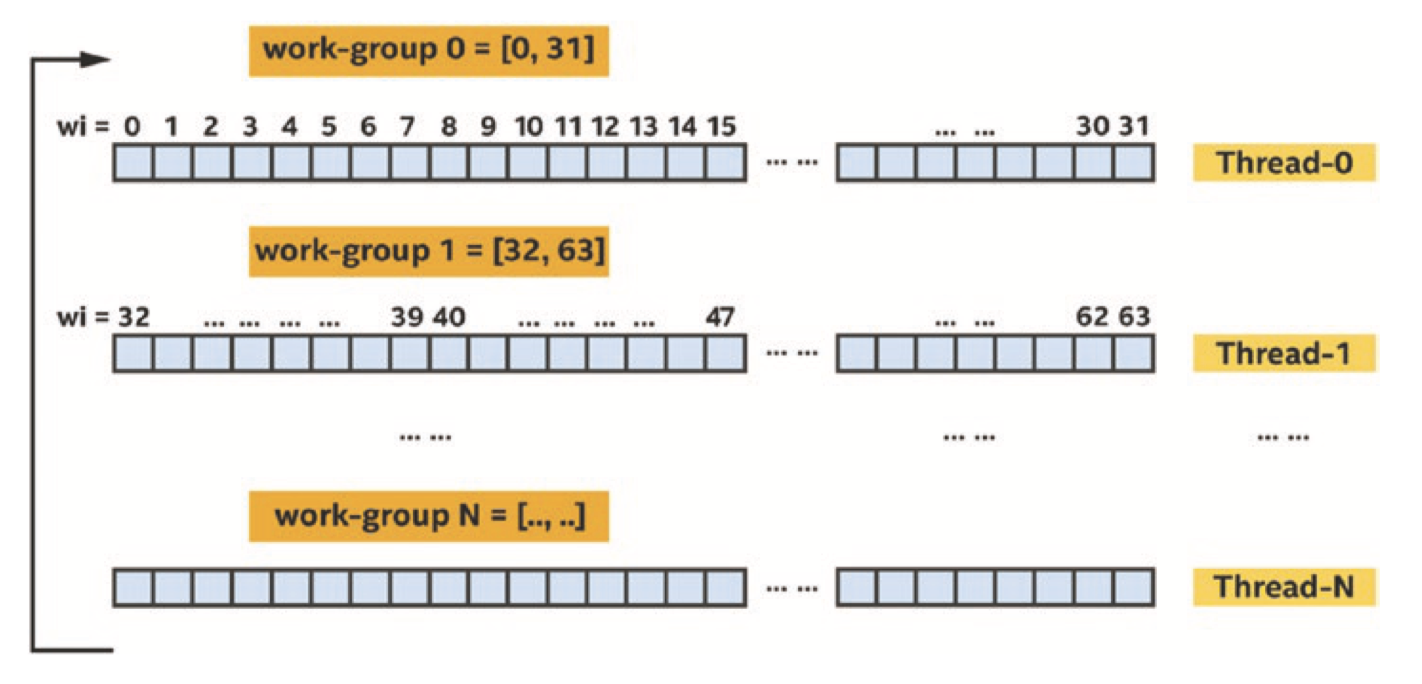
\includegraphics[width=0.9\textwidth]{figs/F16.7.png}
	\caption{\textit{子采样层前向传播路径的顺序 C 实现。 该层还包括激活函数,
	如果卷积层之后没有子采样层,则该激活函数包含在卷积层中。}}
\end{figure}

图 16.7 显示了子采样层前向传播路径的顺序 $\mathrm{C}$ 实现。 
最外面的 $(m)$ for 循环(第 02-11 行)的每次迭代都会生成一个输出特征图。 
接下来的两个级别( $h$ 和 $w$ )的 forloop(第 03-11 行)生成当前输出图的各个像素。 
最里面的两个 for 循环(第 06-09 行)对邻域中的像素进行求和。 
在图 16.4 中的 LeNet-5 子采样示例中,$\mathrm{K}$ 等于 2。 
然后将特定于每个输出特征图的偏差值 b[m] 添加到每个输出特征图,并且总和经过 sigmoid 激活函数。 
读者应该认识到,每个输出像素都是由感知器生成的,该感知器将每个特征图中的四个输入像素作为其输入,
并在相应的输出特征图中生成一个像素。 
ReLU 是另一个常用的激活函数,它是一个简单的非线性滤波器,仅传递非负值:$\mathrm{Y}=\mathrm{X}$,
如果 $\mathrm{X} \geq 0$,否则为 0。

为了完成我们的示例,卷积层 C3 有 16 个输出特征图,每个特征图都是 $10 × 10$ 图像。 
该层有 $6 \times 16=96$ 个滤波器组,每个滤波器组有 $5 \times 5=25$ 权重。 
$\mathrm{C} 3$ 的输出被传递到子采样层 S4,生成 $165 \times 5$ 输出特征图。 
最后,最后一个卷积层 C5 使用 $16 × 120=19205 \times 5$ 滤波器组从其 16 个输入特征图生成 120 个单像素输出特征。

这些特征图通过全连接层 F6,该层有 84 个输出单元,其中每个输出都完全连接到所有输入。 
输出被计算为权重矩阵 $\mathrm{W}$ 与输入向量 $\mathrm{X}$ 的乘积,然后添加偏差并通过 sigmoid 传递输出。 
对于 F6 示例,$\mathrm{W}$ 是一个 $120 \times 84$ 矩阵。 
总之,输出是一个 84 元素向量 Y $6=$ sigmoid $(\mathrm{W} * \mathrm{X}+\mathrm{b})$。 
读者应该认识到,这相当于 84 个感知器,每个感知器将 C5 层生成的所有 120 个单像素 $\mathrm{x}$ 值作为其输入。 
我们将全连接层的详细实现作为练习。

最后阶段是输出层,它使用高斯滤波器生成由十个元素组成的向量,这些元素对应于输入图像包含十个数字之一的概率。

\subsubsection{卷积神经网络反向传播}
CNN 的训练基于第 16.1 节中讨论的随机梯度下降法和反向传播程序(Rumelhart 等人,1986)。 训练数据集标有“正确答案”。 
在手写识别示例中,标签给出了图像中正确的字母。 
标签信息可用于生成最后阶段的“正确”输出:十元素向量的正确概率值,其中正确数字的概率为 1.0 ,所有其他数字的概率为 0.0 。

对于每个训练图像,网络的最后阶段将损失(误差)函数计算为生成的输出概率向量元素值与“正确”输出向量元素值之间的差。 
给定一系列训练图像,我们可以数值计算损失函数相对于输出向量元素的梯度。 
直观上,它给出了当输出向量元素的值发生变化时,损失函数值发生变化的速率。

\begin{figure}[H]
	\centering
	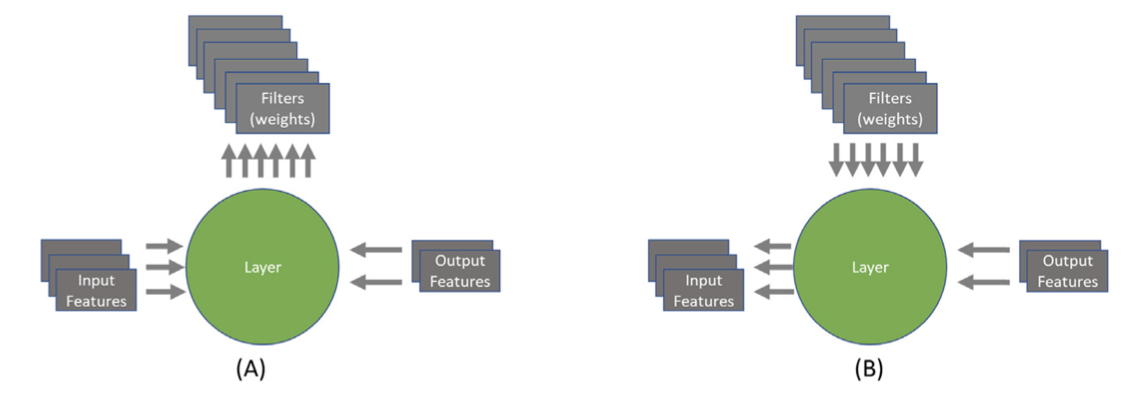
\includegraphics[width=0.9\textwidth]{figs/F16.8.png}
	\caption{\textit{CNN 中层的 (A) $\frac{\partial E}{\partial w}$ 
	和 (B) $\frac{\partial E}{\partial x}$ 的反向传播。}}
\end{figure}

反向传播过程首先计算最后一层损失函数 $\frac{\partial E}{\partial y}$ 的梯度。 
然后,它将梯度从最后一层传播到第一层,穿过网络的所有层。 
每个层接收相对于其输出特征图的 $\frac{\partial E}{\partial y}$ 梯度
作为其输入(这只是后面的 $\frac{\partial E}{\partial x}$ 层)
并计算其自己相对于其输入特征图的$\frac{\partial E}{\partial x}$梯度,如图16.8B所示。 
重复此过程,直到完成网络输入层的调整。

如果一个层已经学习了参数(“权重”)$w$,那么该层还会计算其相对于其权重的 $\frac{\partial E}{\partial w}$ 损失梯度,
如图 16.8 所示 A。 例如,全连接层的形式为 $y=w \cdot x$。 
梯度 $\frac{\partial E}{\partial y}$ 的反向传播由以下等式给出:
$$
\frac{\partial E}{\partial x}=w^{T} \frac{\partial E}{\partial y} \quad \text { and } \quad \frac{\partial E}{\partial w}=\frac{\partial E}{\partial y} x^{T}
$$

这个方程可以在逐个元素的基础上推导,就像我们在两层感知器示例中所做的那样。 
回想一下,每个全连接层输出像素都是由感知器计算的,感知器将输入特征图中的像素作为输入。 
正如我们在第 16.1 节中训练 MLP 时所展示的,输入 $x$ 之一的 $\frac{\partial E}{\partial x}$ 
是 $\frac{\partial E}{\partial y}$ 之间的乘积之和,表示输入元素所贡献的每个输出 $\mathrm{y}$ 元素以及 $w$ 值,
$x$ 值通过该值贡献于 $y$ 值。 因为 $w$ 矩阵的每一行将所有 $x$ 元素(列)与全连接层的 $y$ 元素(其中一行)相关联,
所以 $w$ 的每一列(即 $w 的行) ^{T}$ ) 将所有 $y$ (即 $\frac{\partial E}{\partial y}$ )元素关联回 $x$ (即 $\frac{\partial E}{\partial x}$ ) 元素,因为转置会切换行和列的角色。 
因此,矩阵向量乘法 $w^{T} \frac{\partial E}{\partial y}$ 会产生一个向量,
其所有输入的值均为 $\frac{\partial E}{\partial x}$ $x$ 元素。

类似地,由于每个$w$元素乘以一个$x$元素生成$y$元素,
因此每个w元素的$\frac{\partial E}{\partial w}$可以计算为以下乘积: 
$\frac{\partial E}{\partial y}$ 的元素与 $x$ 元素。 
因此 $\frac{\partial E}{\partial v}$ (单列矩阵)和 $x^{T}$ (单行矩阵)之间的矩阵乘法
会产生 $\frac{\partial E}{\partial w}$ 值。 
这也可以看作 $\frac{\partial E}{\partial y}$ 和 $x$ 向量之间的外积。

让我们将注意力转向卷积层的反向传播。 
我们将从$\frac{\partial E}{\partial y}$开始计算$\frac{\partial E}{\partial x}$,
最终将用于计算上一层的梯度 。 
输入 $x$ 相对于通道 $c$ 的梯度 $\frac{\partial E}{\partial x}$ 给出为与
相应的 $W(m, c) $ 在所有 $m$ 层输出上的“反向卷积”之和:
$$
\frac{\partial E}{\partial x}(c, h, w)=\sum_{m=0}^{M-1} \sum_{p=0}^{K-1} \sum_{q =0}^{K-1}\left(\frac{\partial E}{\partial y}(m, h-p, w-q) * w(m, c, k-p, k-q)\right)
$$

\begin{figure}[H]
	\centering
	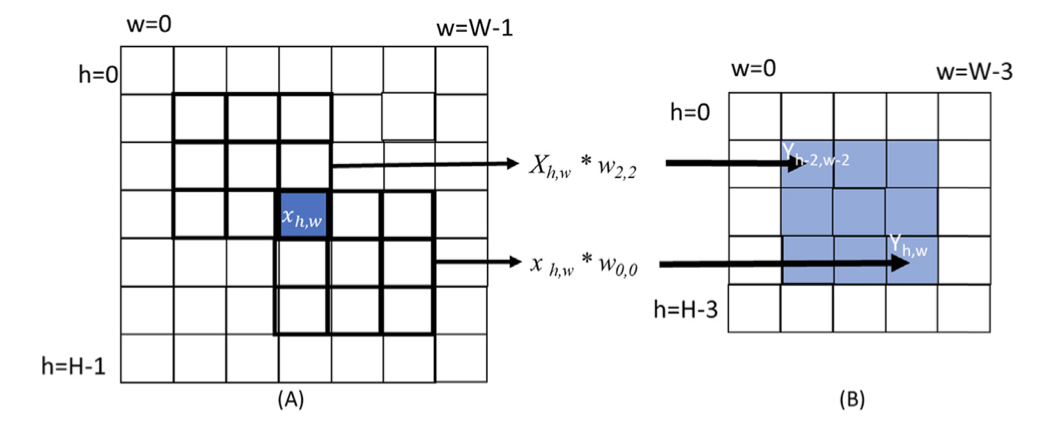
\includegraphics[width=0.9\textwidth]{figs/F16.9.png}
	\caption{\textit{卷积层。 (A) $\frac{\partial E}{\partial w}$ 
	和 (B) $\frac{\partial E}{\partial x}$ 的反向传播。}}
\end{figure}

通过 $h-p$ 和 $w-q$ 索引的后向卷积允许从前向卷积中的 $x$ 元素接收贡献的所有输出 $y$ 元素的梯度,
通过相同的方法为该 $x$ 元素的梯度做出贡献。 重量。 
这是因为在卷积层的前向推理中,$x$元素值的任何变化都会乘以这些$w$元素,并通过这些$y$元素贡献损失函数值的变化。 
图 16.9 显示了使用带有 $3 \times 3$ 滤波器组的小示例的索引模式。 
输出特征图中的九个阴影 $y$ 元素是在前向干扰中接收来自 $x_{h, w}$ 贡献的 $y$ 元素。 
例如,输入元素 $x_{h, w}$ 通过与 $w_{2,2}$ 相乘贡献给 $y_{h-2, w-2}$ 并通过乘法贡献给 $y_{h, w}$ 与 $w_{0,0}$。 
因此,在反向传播过程中,$\frac{\partial E}{\partial \mathrm{x}_{\mathrm{h}, \mathrm{w}}}$应该接收
来自$\frac{\partial E}{\partial y}$ 这九个元素的贡献的值,计算相当于与转置滤波器组 $w^{T}$ 的卷积。

\begin{figure}[H]
	\centering
	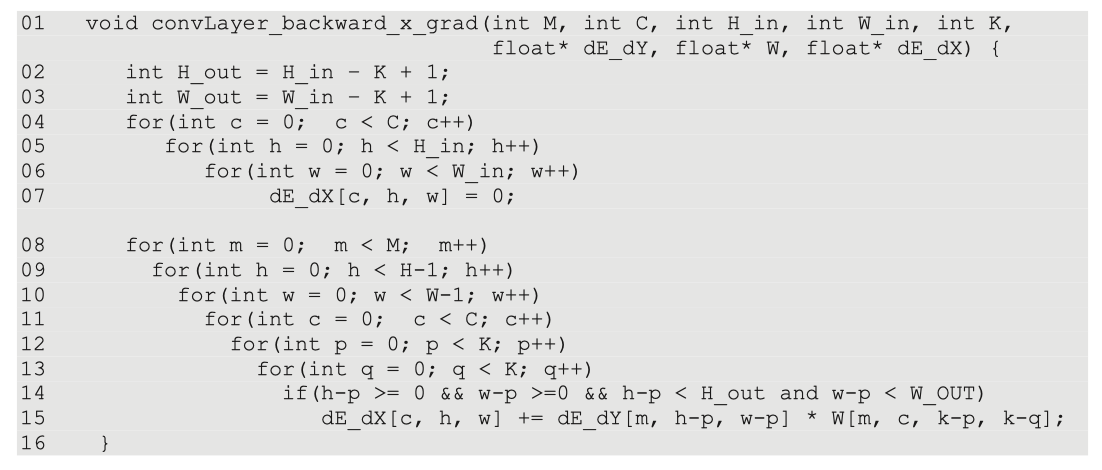
\includegraphics[width=0.9\textwidth]{figs/F16.10.png}
	\caption{\textit{$\frac{\partial E}{\partial x}$ 计算卷积层的后向路径。}}
\end{figure}

图 16.10 显示了用于计算每个输入特征图的 $\frac{\partial E}{\partial x}$ 的每个元素的 $\mathrm{C}$ 代码。 
请注意,代码假设 $\frac{\partial E}{\partial y}$ 已针对该层的所有输出特征图进行了计算,
并通过指针参数 $\mathrm{dE} \_\mathrm{ dY}$。 
这是一个合理的假设,因为当前层的 $\frac{\partial E}{\partial y}$ 
是其紧邻的下一层的 $\frac{\partial E}{\partial x}$,其梯度应该 在到达当前层之前已经在反向传播中计算过了。 
它还假设 $\frac{\partial E}{\partial x}$ 的空间已在设备内存中分配,其句柄作为指针参数 dE\_dX 传入。 
该函数生成 $\frac{\partial E}{\partial x}$ 的所有元素。

\begin{figure}[H]
	\centering
	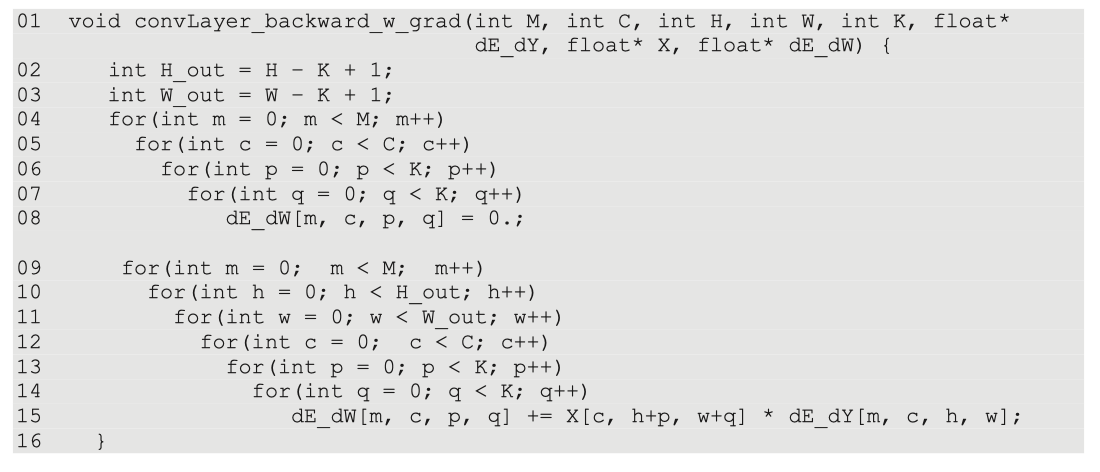
\includegraphics[width=0.9\textwidth]{figs/F16.11.png}
	\caption{\textit{$\frac{\partial E}{\partial w}$ 计算卷积层的后向路径。}}
\end{figure}

卷积层计算 $\frac{\partial E}{\partial w}$ 的顺序代码与 $\frac{\partial E}{\partial x}$ 类似,
如图 16.11 所示 。 由于每个 $W(m, c)$ 都会影响输出 $Y(m)$ 的所有元素,
因此我们应该在相应输出特征图中的所有像素上累积每个 $W(m, c)$ 的梯度:
$$
\frac{\partial E}{\partial W}(m, c, p, q)=\sum_{h=0}^{H_{\text {out }}-1} \sum_{w=0}^ {W_{\text {out }}-1}\left(X(c, h+p, w+q) * \frac{\partial E}{\partial Y}(m, h, w)\right)
$$

请注意,虽然 $\frac{\partial E}{\partial x}$ 的计算对于将梯度传播到前一层很重要,
但 $\frac{\partial E}{\partial w}$ 的计算为 调整当前图层权重值的关键。

计算完所有滤波器组元素位置的 $\frac{\partial E}{\partial w}$ 值后,
使用第 16.1 节中提出的公式更新权重以最小化预期误差: $w \leftarrow w-\varepsilon^{*} \frac{\partial E}{\partial w}$,其中 $\varepsilon$ 是学习率常数。 
$\varepsilon$ 的初始值是根据经验设置的,并根据用户定义的规则通过历元减少。 
$\varepsilon$ 的值在历元中不断减小,以确保权重收敛到最小误差。 
回想一下,调整项的负号会导致变化与梯度方向相反,因此变化可能会减少误差。 
还记得各层的权重值决定输入如何通过网络进行转换。 所有层的这些权重值的调整适应网络的行为。 
也就是说,网络从一系列标记的训练数据中“学习”,并通过调整其所有层的所有权重值来调整其行为,
以适应其推理结果不正确并触发反向传播的输入。

正如我们在第 16.1 节中讨论的,反向传播通常在对训练数据集中的 $N$ 图像的小批量执行前向传递后触发,
并且已计算该小批量的梯度。 使用为小批量计算的梯度更新学习的权重,并用另一个小批量重复该过程。 
\footnote{如果我们按照“优化书”工作,我们应该将使用过的样本返回到训练集,然后通过随机挑选下一个样本来构建新的小批量。 
在实践中,我们按顺序迭代整个训练集。 在机器学习中,训练集的一次传递称为一个纪元。 
然后我们对整个训练集进行洗牌并开始下一个纪元。}
这会向所有先前描述的数组添加一个附加维度,索引为 $n$(小批量中样本的索引)。 
它还在样本上添加了一个额外的循环。

图 16.12 显示了卷积层的修改后的前向路径实现。 它为小批量的所有样本生成输出特征图。

\subsection{卷积层:CUDA 推理内核}
\begin{figure}[H]
	\centering
	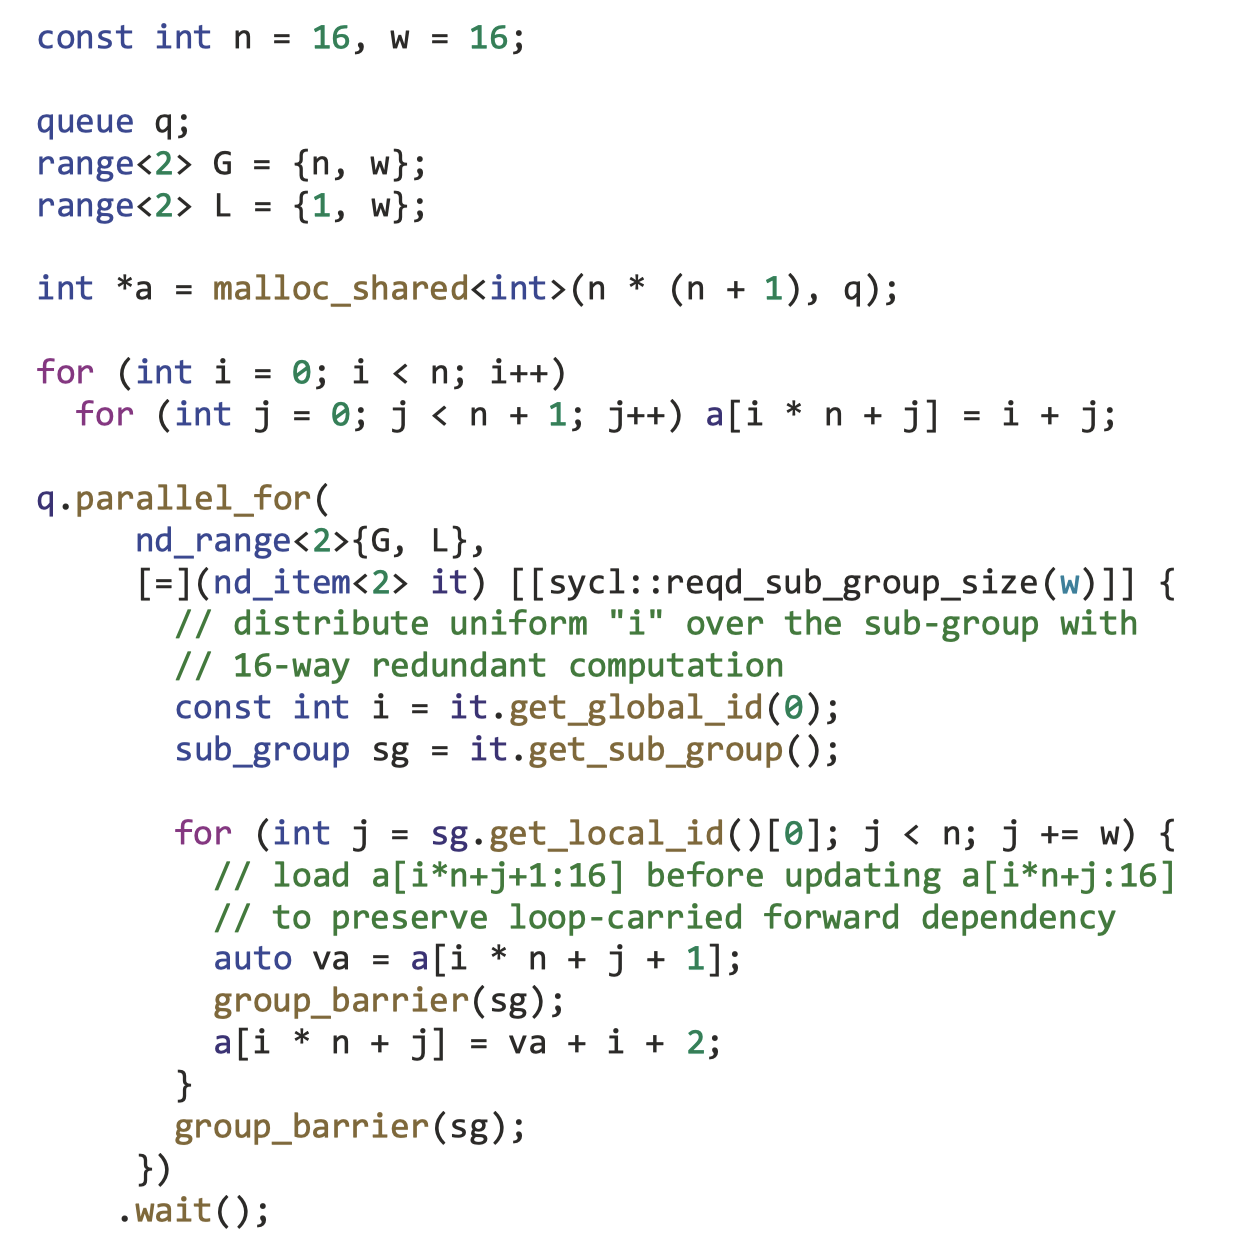
\includegraphics[width=0.9\textwidth]{figs/F16.12.png}
	\caption{\textit{具有小批量训练的卷积层的前向路径。}}
\end{figure}

训练卷积神经网络的计算模式就像矩阵乘法:它既是计算密集型的又是高度并行的。 
我们可以并行处理小批量中的不同样本、同一样本的不同输出特征图以及每个输出特征图的不同元素。 
在图 16.12 中,n 循环(第 04 行,小批量中的样本)、m 循环(第 05 行,输出特征图)
和嵌套 h-w 循环(第 06-07 行,每个输出的像素) 特征图)都是并行循环,因为它们的迭代可以并行执行。 
这四个循环级别一起提供了大规模的并行性。

最里面的三个循环级别,即 c 循环(在输入特征映射或通道上)和嵌套的 p-q 循环(在滤波器组中的权重上),也提供了显着的并行性。 
然而,为了并行化它们,需要使用原子操作来累积到 $Y$ 元素中,
因为这些循环级别的不同迭代可以对相同的 $Y$ 元素执行读取-修改-写入。 
因此,除非我们确实需要更多并行性,否则我们将保持这些循环串行。

假设我们在卷积层中利用四个级别的“简单”并行性 $(n, m, h, w)$,
并行迭代的总数是乘积 $\mathrm{N}^{*} \mathrm{ M}^{*} \mathrm{H} \_$out*W\_out。 
这种高度的可用并行性使卷积层成为 GPU 加速的绝佳候选者。 我们可以轻松地设计一个具有旨在捕获并行性的线程组织的内核。

我们首先需要对线程组织做出一些高层设计决策。 假设我们让每个线程计算一个输出特征图的一个元素。 
我们将使用 2D 线程块,其中每个线程块计算一个输出特征图中 TILE\_WIDTH $\times$ TILE\_WIDTH 像素的图块。 
例如,如果我们设置 TILE\_WIDTH $=16$,则每个块总共有 256 个线程。 
这在处理每个输出特征图的像素时捕获了部分嵌套的 h-w-loop 级并行性。

块可以通过多种不同的方式组织成 3D 网格。 每个选项指定网格尺寸以捕获不同组合中的 $n、m$ 和 $h-w$ 并行度。 
我们将介绍其中一个选项的详细信息,并将其作为练习,供读者探索不同的选项并评估每个选项的潜在利弊。 我们详细介绍的选项如下:
\begin{enumerate}
   \item 第一个维度 $(X)$ 对应于每个块覆盖的 $(M)$ 输出特征图。

   \item 第二个维度 $(Y)$ 反映了输出特征图中块的输出图块的位置。

   \item 网格中的第三个维度 $(Z)$ 对应于小批量中的样本 $(\mathrm{N})$。
\end{enumerate}

\begin{figure}[H]
	\centering
	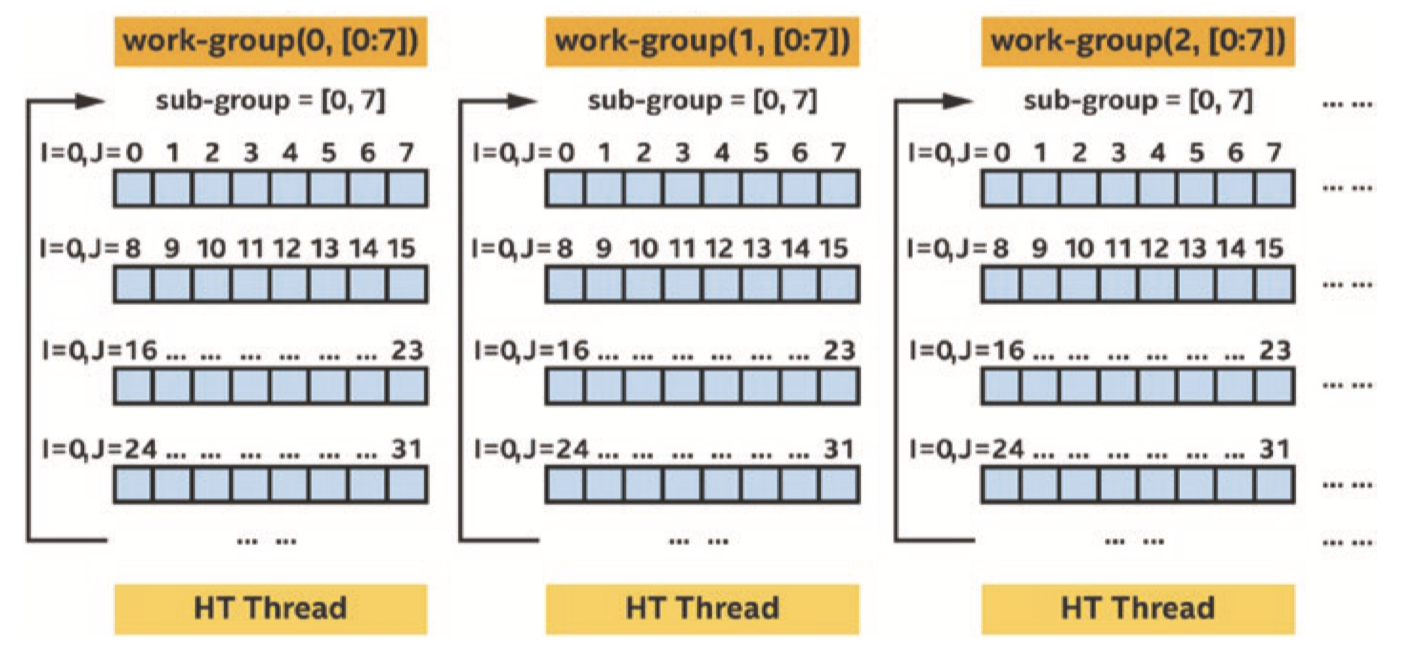
\includegraphics[width=0.9\textwidth]{figs/F16.13.png}
	\caption{\textit{用于启动卷积层内核的主机代码。}}
\end{figure}

图 16.13 显示了基于上面提出的线程组织启动内核的主机代码。 网格的 $X$ 和 $Z$ 维度中的块数很简单; 
它们只是 $M$(输出特征图的数量)和 $N$(小批量中的样本数量)。 $Y$ 维度的排列稍微复杂一些,如图 16.14 所示。 
理想情况下,为了简单起见,我们希望将网格索引的两个维度专用于垂直和水平平铺索引。 
然而,我们只有一个维度,因为我们使用 $X$ 作为输出特征图索引,使用 $Z$ 作为小批量中的样本索引。 
因此,我们对图块索引进行线性化以对输出特征图图块的水平和垂直图块索引进行编码。

\begin{figure}[H]
	\centering
	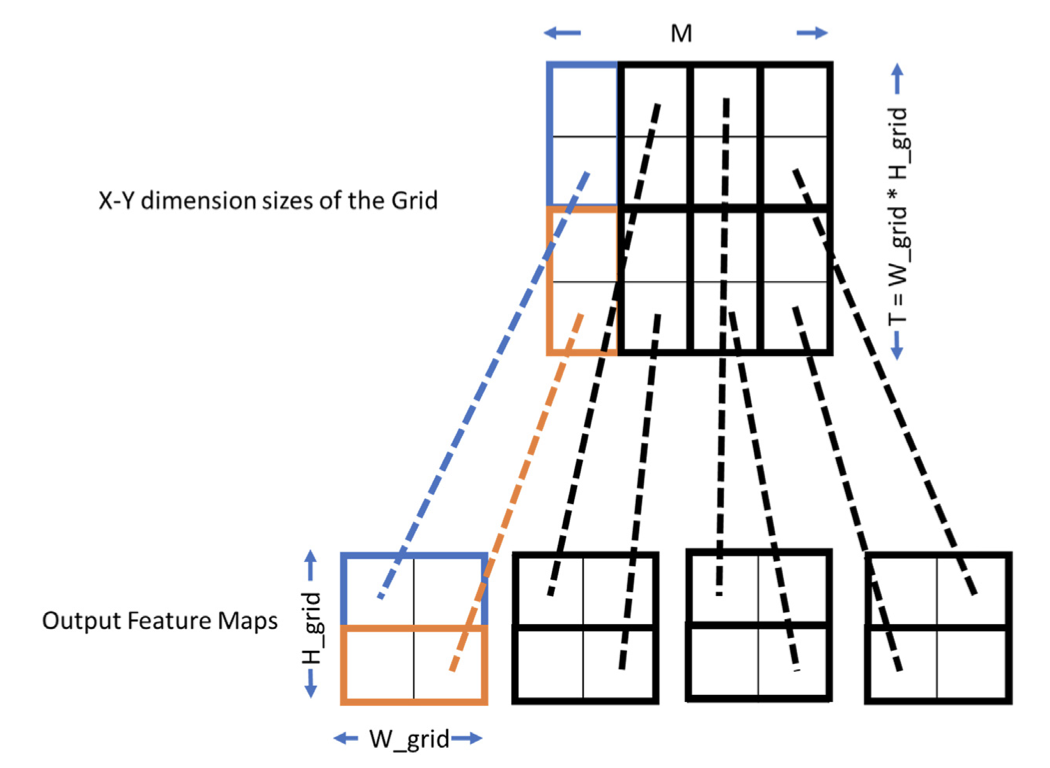
\includegraphics[width=0.9\textwidth]{figs/F16.14.png}
	\caption{\textit{将输出特征图块映射到网格的 X-Y 维度中的块。}}
\end{figure}

在图16.14的例子中,每个样本有四个输出特征图$(M=4)$,
每个输出特征图由$2 \times 2$个tile组成(第02行的H\_grid =2和W\_grid =2 在第 03 行)
每个 $16 \times 16=256$ 像素。 网格组织分配每个块来计算这些图块之一。

我们已经将每个输出特征图分配给$X$维度,这反映为$X$维度中的四个块,每个块对应于一个输出特征图。 
如图 16.14 底部所示,我们对每个输出特征图中的四个图块进行线性化,并将它们分配给 $Y$ 维度中的块。 
因此,图块 (0, 0)、(0, 1)、(1, 0) 和 (1, 1) 使用行主序映射到 blockIdx.y 值分别为 0、1、2 和 3 的块。 
因此,Y 维度中的块总数为 4(第 04 行中的 T = H\_grid × W\_grid = 4)。 
因此,我们将在第 06-07 行启动一个带有 gridDim (4, 4, N) 的网格。

\begin{figure}[H]
	\centering
	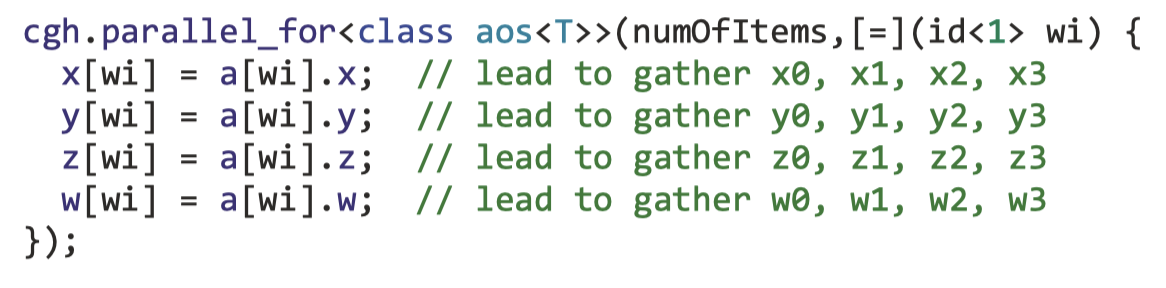
\includegraphics[width=0.9\textwidth]{figs/F16.15.png}
	\caption{\textit{卷积层前向路径的内核。}}
\end{figure}

图 16.15 显示了基于上述线程组织的内核。 请注意,为了清楚起见,在代码中,我们在数组访问中使用多维索引。 
我们让读者将这个伪代码翻译成常规的 $\mathrm{C}$,
假设 $X、Y$ 和 $W$ 必须通过基于行主布局的线性化索引来访问(第 3 章, 多维网格和数据)。

每个线程首先生成其分配的输出特征图像素的 $n$(批量)、$m$(特征图)、$h$(垂直)和 $w$(水平)索引。 
给定主机代码,$n$(第 06 行)和 $m$(第 03 行)索引很简单。 
对于第04行的$h$索引计算,首先将blockIdx.y值除以W\_grid以恢复垂直方向上的图块索引,如图16.13所示。 
然后,该图块索引由 TILE\_WIDTH 扩展并添加到 threadIdx.y,以将实际的垂直像素索引形成到输出特征映射中(第 04 行)。 
水平像素索引的推导类似(第05行)。

图16.15中的内核具有很高的并行性,但消耗了太多的全局内存带宽。 
正如第 7 章“卷积”中有关卷积模式的讨论一样,内核的执行速度将受到全局内存带宽的限制。 
正如我们在第 7 章“卷积”中看到的,我们可以使用恒定内存缓存和共享内存平铺来显着减少全局内存流量并提高内核的执行速度。 
这些对卷积推理内核的优化留给读者作为练习。

\subsection{将卷积层表示为 GEMM}
我们可以通过将其表示为等效的矩阵乘法运算,
然后使用 CUDA 线性代数库 cuBLAS 中的高效 GEMM(通用矩阵乘法)内核来构建更快的卷积层。 
该方法由 Chellapilla 等人提出。 (2006)。 
中心思想是以这样一种方式展开和复制输入特征图像素,即计算一个输出特征图像素所需的所有元素将存储为由此产生的矩阵的一个连续列。 
这将卷积层的前向运算表述为一个大矩阵乘法。
\footnote{另请参阅 https://petewarden.com/2015/04/20/why-gemm-is-at-the-heart-of-deep-learning/ 了解非常详细的解释。}

考虑一个小示例卷积层,它采用 $C=3$ 特征图作为输入,每个特征图的大小为 $3 \times 3$,并生成 $M=2$ 输出特征,
每个特征图的大小为 $2 \times 2 $,如图 16.5 所示,为方便起见,位于图 16.16 顶部。 
它使用 $M \times C=6$ 个滤波器组,每个滤波器组为 $2 \times 2$。 该层的矩阵版本将按以下方式构建。

\begin{figure}[H]
	\centering
	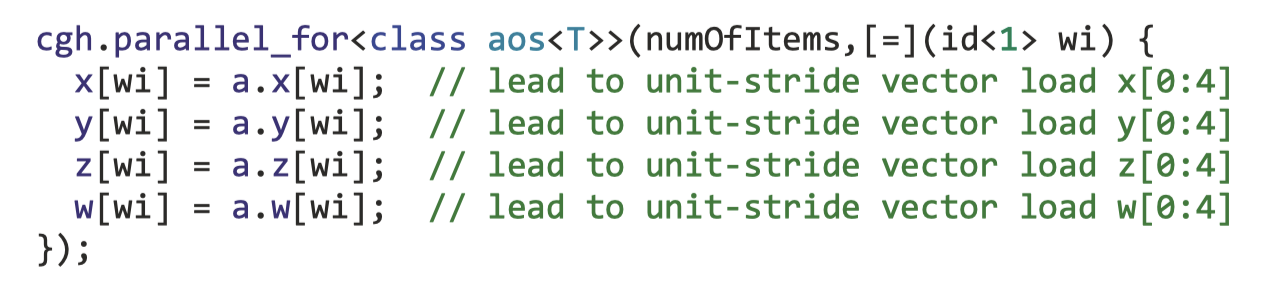
\includegraphics[width=0.9\textwidth]{figs/F16.16.png}
	\caption{\textit{将卷积层表述为 GEMM。}}
\end{figure}

首先,我们将重新排列所有输入像素。 由于卷积的结果是跨输入特征求和的,因此输入特征可以连接成一个大矩阵。 
每个输入特征图成为大矩阵中的行的一部分。 
如图16.16所示,输入特征图0、1和2分别成为“输入特征X\_unrolled”矩阵的顶部、中间和底部部分。

重新排列后,结果矩阵的每一列都包含计算输出特征的一个元素所需的所有输入值。 
例如,在图16.16中,计算输出特征图0的$(0,0)$处的值所需的所有输入特征像素都在输入特征图中圈出:
$$
\begin{aligned}
Y_{0,0,0} & =(1,2,1,1) \cdot(1,1,2,2)+(0,2,0,3) \cdot(1,1,1,1 )+(1,2,0,1) \cdot(0,1,1,0) \\
& =1+2+2+2+0+2+0+3+0+2+0+0 \\
&=14
\end{aligned}
$$

其中每个内积的第一项是通过对图 16.16 中圈出的 $x$ 像素块进行线性化而形成的向量。 
第二项是通过对用于卷积的滤波器组进行线性化而形成的向量。 在这两种情况下,线性化都是通过使用行优先顺序来完成的。 
同样清楚的是,我们可以将三个内积重新表示为一个内积:
$$
\begin{aligned}
Y_{0,0,0} & =(1,2,1,1,0,2,0,3,1,2,0,1) \cdot(1,1,2,2,1,1, 1,1,0,1,1,0) \\
& =1+2+2+2+0+2+0+3+0+2+0+0 \\
&=14
\end{aligned}
$$

如图 16.16 底部所示,来自滤波器组的串联向量成为滤波器矩阵的第 0 行,
来自输入特征图的串联向量成为输入特征图展开矩阵的第 0 列。 
在矩阵乘法期间,滤波器组矩阵的行和输入特征矩阵的列将产生输出特征图的一个像素。

请注意,$2 \times 12$ 过滤器矩阵和 $12 \times 8$ 输入特征图矩阵的矩阵乘法会生成 $2 \times 8$ 输出特征图矩阵。 
输出特征图矩阵的顶部是输出特征图 0 的线性化形式,底部是输出特征图 1。
两者都已经按行优先顺序排列,因此它们可以用作下一个的单独输入特征图 层。 
对于滤波器组,滤波器矩阵的每一行只是原始滤波器组的行主阶视图。 
因此,滤波器矩阵只是所有原始滤波器组的串联。 不涉及过滤元件的物理重新排列或重新定位。

我们进行了一个重要的观察,由于卷积的性质,用于计算输出特征图不同像素的输入特征图像素块彼此重叠。 
这意味着当我们生成扩展的输入特征矩阵时,每个输入特征图像素都会被复制多次。 
例如,每个 $3 \times 3$ 输入特征图的中心像素被使用四次来计算输出特征的四个像素,因此它将被复制四次。 
每条边缘上的中间像素被使用两次,因此它将被复制两次。 每个输入特征角上的四个像素仅使用一次,不需要重复。 
因此扩展后的输入特征矩阵部分的像素总数为$4 * 1+2 * 4+$ $1 * 4=16$。 
由于每个原始输入特征图只有 9 个像素,因此 GEMM 公式会产生 $16 / 9=1.8$ 的扩展比率来表示输入特征图。

一般来说,展开的输入特征图矩阵的大小可以从生成每个输出特征图元素所需的输入特征图元素的数量导出。 
扩展矩阵的高度或行数是对每个输出特征图元素有贡献的输入特征元素的数量,
即 $\mathrm{C}^{*} \mathrm{~K}^{*} \mathrm{~K}$ :
每个输出元素是来自每个输入特征映射的 $\mathrm{K}^{*} \mathrm{~K}$ 个元素的卷积,
并且有 $\mathrm{C}$ 个输入特征 地图。 在我们的示例中,$\mathrm{K}$ 为 2,
因为滤波器组为 $2 \times 2$ 并且存在三个输入特征图。 
因此,扩展后的矩阵的高度应为$3 * 2 * 2=12$,这正是图16.16所示矩阵的高度。

扩展矩阵的宽度或列数是每个输出特征图中的元素数量。 
如果每个输出特征图是一个 H\_out $\times$ W\_out 矩阵,则扩展矩阵的列数为 H\_out*W\_out。 
在我们的示例中,每个输出特征图都是一个 $2 \times 2$ 矩阵,在扩展矩阵中产生四列。 
请注意,输出特征图 $M$ 的数量不会影响重复。 这是因为所有输出特征图都是根据相同的扩展输入特征图矩阵计算的。

输入特征图的扩展比率是扩展矩阵的大小与原始输入特征图的总大小之比。 读者应验证扩展比如下:
$$
\frac{\mathrm{C} * \mathrm{~K} * \mathrm{~K} * \mathrm{H} \_ \text {out } * \mathrm{~W} \_ \text {out }} {\mathrm{C} * \mathrm{H} \_ \text {在} * \mathrm{~W} \_ \text {在}}
$$

其中 $\mathrm{H} \_$in 和 $\mathrm{W}$ \_in 分别是每个输入特征图的高度和宽度。 
在我们的示例中,比率为 $(3 * 2 * 2 * 2 * 2) /(3 * 3 * 3)=16 / 9$。 
一般来说,如果输入特征图和输出特征图远大于滤波器组,则扩展比率将接近 $\mathrm{K}^{*} \mathrm{~K}$。 
滤波器组表示为完全线性化布局中的滤波器组矩阵,其中每一行包含生成一个输出特征图所需的所有权重值。 
滤波器组矩阵的高度是输出特征图$(M)$的数量。 计算不同的输出特征图涉及共享单个扩展的输入特征图矩阵。 
滤波器组矩阵的宽度是生成每个输出特征图元素所需的权重值的数量,
即 $\mathrm{C}^{*} \mathrm{~K}^{*} \mathrm{~ K}$。 回想一下,将权重值放入滤波器组矩阵时不会出现重复。 
例如,滤波器组矩阵只是图 16.16 中六个滤波器组的串联排列。

当我们将滤波器组矩阵 $W$ 乘以扩展的输入矩阵 X\_unrolled 时,
输出特征图将计算为高度 $M$ 和宽度 H\_out*W\_out 的矩阵 $Y$。 即$Y$的每一行都是一个完整的输出特征图。

现在让我们讨论如何在 CUDA 中实现该算法。 我们首先讨论数据布局。 
我们可以从输入和输出矩阵的布局开始。
\begin{itemize}
   \item 我们假设小批量中的输入特征图样本将以与基本 CUDA 内核相同的方式提供。 
   	它被组织为 $\mathrm{N}$ $\times \mathrm{C} \times \mathrm{H} \times \mathrm{W}$ 数组,
   	其中 $\mathrm{N}$ 是样本数 在小批量中,$\mathrm{C}$是输入特征图的数量,
   	$\mathrm{H}$是每个输入特征图的高度,$\mathrm{W}$是每个输入特征图的宽度 地图。

   \item 如图 16.16 所示,矩阵乘法自然会产生一个输出 Y,
   	存储为 $\mathrm{M} \times\left(\mathrm{H} \_\right.$out ${ }^{ *} \mathrm{~W} \_$out $)$数组。 
   	这就是原始的基本 CUDA 内核将产生的结果。

   \item 由于滤波器组矩阵不涉及权重值的重复,
   	因此我们假设它将提前准备好
   	并组织为 $\mathrm{M} \times \mathrm{C} \times$ $\mathrm{K }^{2}$ 数组如图 16.16 所示。
\end{itemize}

展开的输入特征图矩阵$X_{-}$unroll的准备更加复杂。 由于每次扩展都会将输入大小增加 $\mathrm{K}^{2}$ 倍,
因此对于 5 或更大的典型 $\mathrm{K}$ 值,扩展比率可能非常大。 用于保存小批量的所有样本输入特征图的内存占用可能会非常大。
为了减少内存占用,我们将只为 X\_unrolled [C * K * K * H\_out * W\_out] 分配一个缓冲区。 
我们将通过循环小批量中的样本来重用该缓冲区。 在每次迭代期间,我们将样本输入特征图从其原始形式转换为展开矩阵。

\begin{figure}[H]
	\centering
	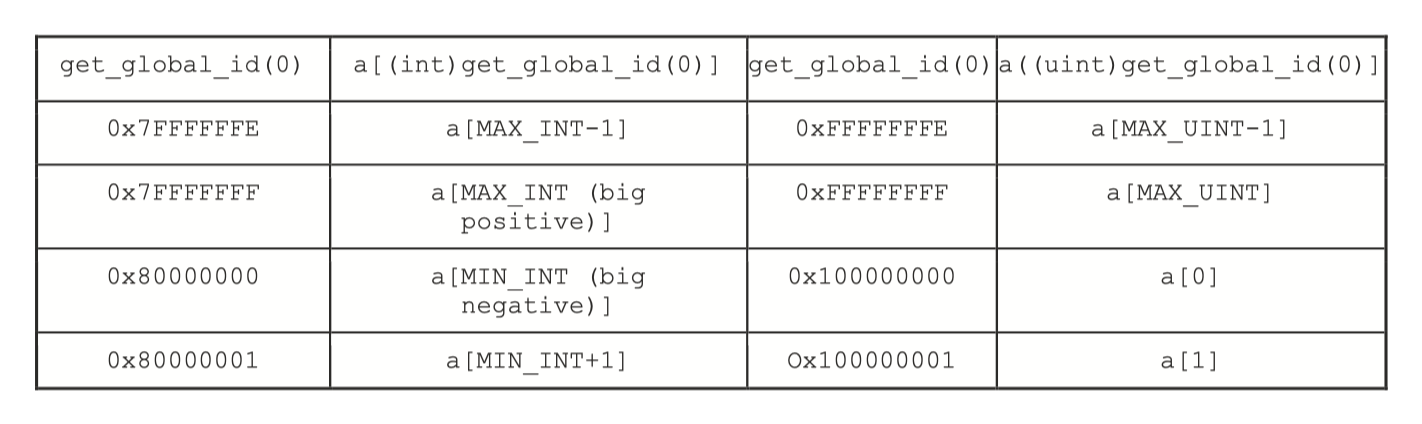
\includegraphics[width=0.9\textwidth]{figs/F16.17.png}
	\caption{\textit{生成展开的 X 矩阵的 C 函数。 为了清楚起见,数组访问采用多维索引形式,
	并且需要线性化以使代码可编译。}}
\end{figure}

图 16.17 显示了一个顺序函数,它通过收集和复制输入特征图 $\mathrm{X}$ 的元素来生成 $\mathrm{X}$ \_unroll 数组。 
该函数使用五级循环。 最里面的两层 for 循环($w$ 和 $h$,第 08-13 行)为每个输出特征映射元素放置一个输入特征映射元素。 
接下来的两个级别($p$ 和 $q$,第 06-14 行)对每个 $\mathrm{K}^{*} \mathrm{~K}$ 过滤矩阵元素重复该过程。 
最外面的循环重复所有输入特征图的过程。 这种实现在概念上很简单,并且可以很容易地并行化,因为循环不会在其迭代之间强加依赖性。 
此外,最内层循环(w,第 10-13 行)的连续迭代从 $\mathrm{X}$ 中输入特征图之一的局部图块读取,
并写入到连续位置(X\_unroll 中的同一行) 扩展矩阵 X\_unroll。 这应该会导致 CPU 上内存带宽的高效使用。

我们现在准备设计一个 CUDA 内核来实现输入特征图展开。 
每个 CUDA 线程将负责从一个输入特征映射中收集 $\left(\mathrm{K}^{*} \mathrm{~K}\right)$ 输入元素,
作为输出特征映射的一个元素。 
线程总数为 $\left(\mathrm{C}^{*} \mathrm{H} \_\right.$out ${ }^{*} \mathrm{~W}$ \_out $) $。 
我们将使用一维线程块并从线性化线程索引中提取多维索引。

\begin{figure}[H]
	\centering
	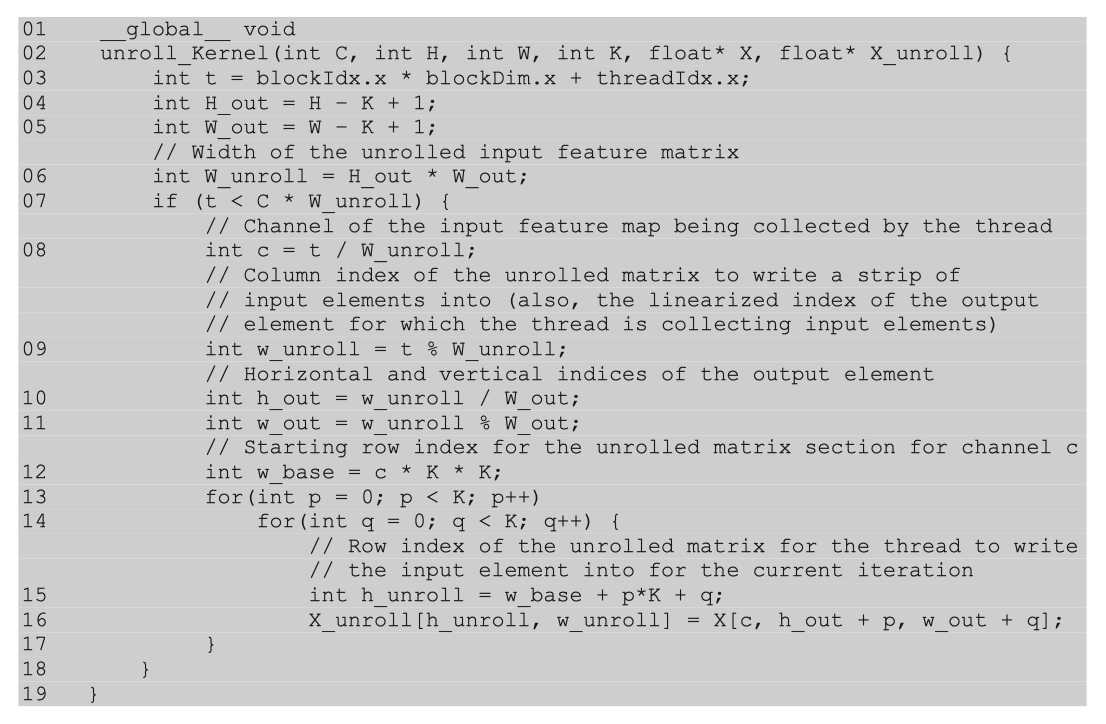
\includegraphics[width=0.9\textwidth]{figs/F16.18.png}
	\caption{\textit{用于展开输入特征图的 CUDA 内核实现。 
	为了清楚起见,数组访问采用多维索引形式,并且需要线性化以使代码可编译。}}
\end{figure}

图 16.18 显示了展开内核的实现。 请注意,每个线程都会构建列的 $\mathrm{K}^{*} \mathrm{~K}$ 部分,
如图 16.16 中的输入要素 X\_Unrolled 数组中的阴影框所示。 
每个这样的部分包含来自通道 $\mathrm{c}$ 的输入特征图 $\mathrm{X}$ 的补丁的所有元素,
这是与相应滤波器执行卷积运算以产生输出 Y 的一个元素所需的。

比较图16.17和16.18的循环结构,图16.17中最里面的两个循环级别已更改为图16.18中的外部级别循环。 
这种交换允许收集计算输出元素所需的输入元素的工作由多个线程并行完成。 
此外,让每个线程从输入特征图中收集生成输出所需的所有输入特征图元素会生成合并的存储器写入模式。 
如图 16.16 所示,相邻线程将在一行中写入相邻的 $\mathrm{X}$ \_unroll 元素,因为它们都垂直移动以完成其部分。 
对 $X$ 的读取访问模式类似,可以通过检查相邻线程的 w\_out 值来分析。 我们将对读取访问模式的详细分析留作练习。

一个重要的高级假设是我们将输入特征图、滤波器组权重和输出特征图保存在设备内存中。 
滤波器组矩阵准备一次并存储在设备全局存储器中以供所有输入特征图使用。 
对于小批量中的每个样本,我们启动 unroll\_Kernel 来准备扩展矩阵并启动矩阵乘法内核,如图 16.16 所示。

通过矩阵乘法实现卷积可以非常高效,因为矩阵乘法在所有硬件平台上都经过了高度优化。 
矩阵乘法在 GPU 上特别快,因为它在全局内存数据访问的每个字节中具有很高的浮点运算比率。 
该比率随着矩阵变大而增加,这意味着矩阵乘法在小矩阵上效率较低。 因此,这种卷积方法在创建大型乘法矩阵时最为有效。

正如我们之前提到的,滤波器组矩阵是一个 $\mathrm{M} \times(\mathrm{C} * \mathrm{~K} * \mathrm{~K})$ 矩阵,
扩展后的输入特征图矩阵是 $(\mathrm{C} * \mathrm{~K} * \mathrm{~K}) \times\left(\mathrm{H} \_\right.$out $* \mathrm{~W} \_ $out $)$ 矩阵。 
请注意,除了滤波器组矩阵的高度外,所有维度的大小都取决于参数与卷积的乘积,而不是参数本身。 
虽然单个参数可能很小,但它们的乘积往往很大。 
例如,在卷积网络的早期层中,$\mathrm{C}$ 很小,但 $\mathrm{H} \_$out 和 W\_out 很大。 
另一方面,在网络末端,$\mathrm{C}$很大,但H\_out和W\_out很小。 
因此,对于所有层来说,乘积 $\mathrm{C}^{*} \mathrm{H} \_$out*${ }^{*} \mathrm{~W} \_o u t$ 通常都很大。 
这意味着所有层的矩阵大小往往都很大,因此使用这种方法的性能往往很高。

形成扩展输入特征映射矩阵的一个缺点是,它涉及将输入数据复制高达 $\mathrm{K}^{*} \mathrm{~K}$ 次,
这可能需要分配大量的 记忆。 为了解决这个限制,如图 16.16 所示的实现逐块具体化 X\_unroll 矩阵,
例如,通过形成扩展的输入特征映射矩阵并为小批量的每个样本迭代调用矩阵乘法。 
然而,这限制了实现中的并行性,有时会导致矩阵乘法太小而无法有效利用 GPU。 
这种公式的另一个缺点是它降低了卷积的计算强度,因为除了读取 $\mathrm{X}$ 本身之外,还必须写入和读取 X\_unroll,
这比直接方法需要更多的内存流量。 因此,最高性能的实现在实现展开算法时具有更复杂的安排,
以最大限度地提高 GPU 利用率,同时保持对 DRAM 的读取最少。 当我们在下一节中介绍 CUDNN 方法时,我们将回到这一点。

\subsection{CUDNN库}
CUDNN 是一个用于实现深度学习原语的优化例程库。 它旨在让深度学习框架更轻松地利用 GPU。 
它提供了灵活且易于使用的 C 语言深度学习 API, 
可以巧妙地集成到现有的深度学习框架(例如 Caffe、Tensorflow、Theano、Torch)中。 
正如我们在上一节中讨论的那样,该库要求输入和输出数据驻留在 GPU 设备内存中。 
此要求类似于 cuBLAS 的要求。

该库是线程安全的,因为它的例程可以从不同的主机线程调用。 前向和后向路径的卷积例程使用封装层属性的通用描述符。 
张量和过滤器通过不透明描述符访问,可以灵活地使用沿每个维度的任意步幅指定张量布局。 
$\mathrm{CNN}$ 中最重要的计算原语是一种特殊形式的批量卷积。 
在本节中,我们描述该卷积的前向形式。 表 16.1 列出了控制该卷积的 CUDNN 参数。

\begin{figure}[H]
	\centering
	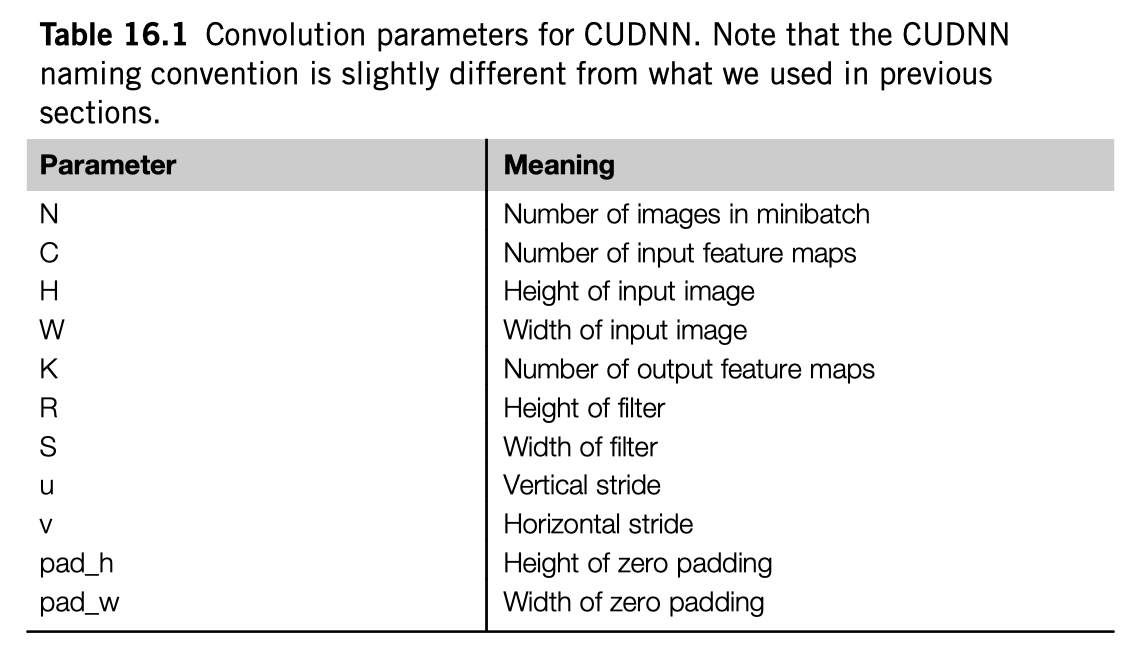
\includegraphics[width=0.9\textwidth]{figs/F16-table.png}
\end{figure}

卷积有两个输入:
\begin{enumerate}
   \item $\mathrm{D}$ 是一个四维 $\mathrm{N} \times \mathrm{C} \times \mathrm{H} \times \mathrm{W}$ 张量,其中包含输入数据。
   \footnote{张量是一个数学术语,表示二维以上的数组。 在数学中,矩阵只有二维。 
   具有三个或更多维度的数组称为张量。 就本书而言,T 维张量可以简单地视为 T 维数组。}

   \item $\mathrm{F}$ 是一个四维 $\mathrm{K} \times \mathrm{C} \times \mathrm{R} \times \mathrm{S}$ 张量,其中包含卷积滤波器。
\end{enumerate}

输入数据数组(张量)$\mathrm{D}$ 的范围超过小批量中的 $\mathrm{N}$ 个样本,
每个样本 $\mathrm{C}$ 输入特征映射,每个 $\mathrm{H}$ 行 输入特征图,以及每个输入特征图的 $\mathrm{W}$ 列。 
滤波器范围涵盖 $\mathrm{K}$ 输出特征图、$\mathrm{C}$ 输入特征图、每个滤波器组 $\mathrm{R}$ 行以及每个滤波器组 $\mathrm{S}$ 列 。 
输出也是一个四维张量 $\mathrm{O}$,其范围超过小批量中的 $\mathrm{N}$ 个样本,$\mathrm{K}$ 输出特征图,
每个输出 $\mathrm{P}$ 行 特征图,以及每个输出特征图的 $\mathrm{Q}$ 列,
其中 $\mathrm{P}=\mathrm{f}(\mathrm{H} ; \mathrm{R} ; \mathrm{u} ;$ pad\_h $)$ 
和 $\mathrm{Q}=\mathrm{f}(\mathrm{W} ; \mathrm{S} ; \mathrm{v}$; pad\_w $)$,
表示高度 输出特征图的宽度和宽度取决于输入特征图和滤波器组的高度和宽度,以及填充和跨步选择。 
跨步参数 $\mathrm{u}$ 和 $\mathrm{v}$ 允许用户通过仅计算输出像素的子集来减少计算负载。 
填充参数允许用户指定将多少行或列的 0 条目附加到每个特征映射,以改进内存对齐和/或矢量化执行。

CUDNN (Chetlur et al., 2014) 支持用于实现卷积层的多种算法:基于矩阵乘法的 GEMM (Tan et al., 2011) 
和 Winograd (Lavin \& Scott, 2016)、基于 FFT (Vasilache et al., 2016) ,2014),等等。 
使用矩阵乘法实现卷积的基于 GEMM 的算法类似于 16.4 节中介绍的方法。 
正如我们在第 16.4 节末尾所讨论的,在全局内存中具体化扩展的输入特征矩阵在全局内存空间和带宽消耗方面可能代价高昂。 
CUDNN 通过延迟生成扩展输入特征图矩阵 X\_unroll 并将其加载到片上存储器中来避免此问题,
而不是在调用矩阵乘法例程之前将其收集到片外存储器中。 
NVIDIA 提供了基于矩阵乘法的例程,可实现 GPU 上最大理论浮点吞吐量的高利用率。 
该例程的算法与 Tan 等人描述的算法类似。 (2011)。 
输入矩阵 A 和 B 的固定大小子矩阵被连续读入片上存储器,然后用于计算输出矩阵 C 的子矩阵。
由卷积带来的所有索引复杂性都在瓦片管理中处理 这个例程。 
我们对 A 和 B 的图块进行计算,同时将 A 和 B 的下一个图块从片外存储器提取到片上缓存和其他存储器中。 
该技术隐藏了与数据传输相关的内存延迟,使得矩阵乘法计算仅受执行算术计算所需的时间的限制。


由于矩阵乘法例程所需的平铺与卷积的任何参数无关,因此 $\mathrm{X}_{-}$unroll 的平铺边界与卷积问题之间的映射是重要的。 
因此,CUDNN 方法需要计算此映射并使用它来将 A 和 B 的正确元素加载到片上存储器中。 
随着计算的进行,这种情况会动态发生,这使得 CUDNN 卷积实现能够利用优化的基础设施进行矩阵乘法。 
与矩阵乘法相比,它需要额外的索引算术,但它充分利用矩阵乘法的计算引擎来执行工作。 
计算完成后,CUDNN 执行所需的张量转置,将结果存储在用户所需的数据布局中。

\subsection{总结}
本章首先简要介绍了机器学习。 然后,它更深入地研究分类任务并引入感知器,这是一种线性分类器,是理解现代 CNN 的基础。 
我们讨论了如何为单层和 MLP 实现前向推理和后向传播训练过程。 
特别是,我们讨论了对可微激活函数的需求,以及在训练过程中如何通过多层感知器网络中的链式规则更新模型参数。

基于对感知器的概念和数学理解,我们提出了一个基本的卷积神经网络及其主要类型层的实现。 
这些层可以被视为感知器的特殊情况和/或简单改编。 
然后,我们在第 7 章“卷积”中的卷积模式的基础上,提出了卷积层(CNN 中计算最密集的层)的 CUDA 内核实现。

然后,我们提出了通过将输入特征映射展开为矩阵来将卷积层公式化为矩阵乘法的技术。 
该转换使卷积层能够从针对 GPU 的高度优化的 GEMM 库中受益。 
我们还介绍了输入矩阵展开过程的 C 和 CUDA 实现,并讨论了展开方法的优缺点。

我们在本章结束时概述了大多数深度学习框架都使用的 CUDNN 库。 
这些框架的用户可以从高度优化的层实现中受益,而无需自己编写 CUDA 内核。